% ============================================================
% AI-BOM Architecture & Schema Specification — Master Slides
% Style: Clear Dev-Speak with Rich Practical Examples & Zero Overflow
% ============================================================

\documentclass[aspectratio=169, xcolor=table]{beamer}

% load pkgs & styling
% pkg config

% req pkgs
\usepackage[utf8]{inputenc}
\usepackage[T1]{fontenc}
\usepackage[english]{babel}

% clean modern font (available in all LaTeX distributions)
\usepackage{lmodern}

% math stuff
\usepackage{amsmath}
\usepackage{amssymb}
\usepackage{mathtools}
\usepackage{bm}

% pics & figs
\usepackage{graphicx}
\usepackage{subcaption}

% tbls
\usepackage{booktabs}
\usepackage{multirow}
\usepackage{array}

% draw nn & charts
\usepackage{tikz}
\usetikzlibrary{shapes, arrows.meta, positioning, calc, shadows, decorations.pathreplacing, backgrounds}
\usepackage{pgfplots}
\pgfplotsset{compat=1.18}

% code
\usepackage{listings}
\usepackage{xcolor}

% icons
\usepackage{fontawesome5}

% premium ui blocks
\usepackage[most]{tcolorbox}

% biblio (uncomment & add references.bib to enable)
%\usepackage[backend=biber,style=authoryear,maxnames=2,natbib=true]{biblatex}
%\addbibresource{references.bib}

% appendix section helper
\usepackage{appendixnumberbeamer}

% color palette
\definecolor{myprimary}{HTML}{1A365D} % deep navy
\definecolor{myaccent}{HTML}{0D9488}  % teal
\definecolor{mygreen}{HTML}{059669}   % emerald
\definecolor{mygrey}{HTML}{F1F5F9}    % slate grey

% ============================================================
% tcolorbox ui components
% ============================================================

% modern info block
\newtcolorbox{infobox}[1][]{
    enhanced,
    colback=myprimary!4,
    colframe=myprimary,
    boxrule=0.5pt,
    leftrule=3.5pt,
    arc=3pt,
    boxsep=2pt,
    top=4pt,bottom=4pt,left=6pt,right=6pt,
    drop fuzzy shadow,
    fonttitle=\bfseries,
    coltitle=myprimary,
    colbacktitle=myprimary!4,
    title=#1
}

% modern alert block
\newtcolorbox{alertbox}[1][]{
    enhanced,
    colback=myaccent!5,
    colframe=myaccent,
    boxrule=0.5pt,
    leftrule=3.5pt,
    arc=3pt,
    boxsep=2pt,
    top=4pt,bottom=4pt,left=6pt,right=6pt,
    drop fuzzy shadow,
    fonttitle=\bfseries,
    coltitle=myaccent,
    colbacktitle=myaccent!5,
    title=#1
}

% modern success block
\newtcolorbox{successbox}[1][]{
    enhanced,
    colback=mygreen!4,
    colframe=mygreen,
    boxrule=0.5pt,
    leftrule=3.5pt,
    arc=3pt,
    boxsep=2pt,
    top=4pt,bottom=4pt,left=6pt,right=6pt,
    drop fuzzy shadow,
    fonttitle=\bfseries,
    coltitle=mygreen,
    colbacktitle=mygreen!4,
    title=#1
}


% metropolis theme config
\usetheme[progressbar=frametitle,block=transparent,titleformat=smallcaps]{metropolis}

% colors
\setbeamercolor{normal text}{fg=darkgray,bg=white}
\setbeamercolor{frametitle}{bg=myprimary,fg=white}
\setbeamercolor{progress bar}{fg=myaccent,bg=myprimary!40}
\setbeamercolor{alerted text}{fg=myaccent}

% compact frametitle
\setbeamerfont{frametitle}{size=\large,series=\bfseries}
\makeatletter
\setbeamertemplate{frametitle}{%
    \nointerlineskip%
    \begin{beamercolorbox}[wd=\paperwidth,sep=0pt]{frametitle}%
        \hspace*{12pt}%
        \parbox[c][22pt][c]{\dimexpr\paperwidth-24pt\relax}{%
            \usebeamerfont{frametitle}\insertframetitle%
        }%
    \end{beamercolorbox}%
    \usebeamertemplate*{progress bar in head/foot}%
}
\makeatother

% footer
\setbeamertemplate{footline}{%
    \hfill%
    \usebeamerfont{page number in head/foot}%
    \textcolor{myprimary!70}{\insertframenumber\,/\,\inserttotalframenumber}%
    \hspace*{8pt}\vspace{4pt}%
}

% metadata
\title[AI-BOM Architecture \& Schema]{AI-BOM Architecture \& Schema Specification}
\subtitle{Evidence-Based Identity, Two-Tier Storage \& CycloneDX 1.6 ML-BOM}
\author[AI-BOM Core Team]{\textbf{AI-BOM - SCA}}
\institute[OPSWAT R\&D]{AI Software Bill of Materials Engine 0.1.0 · Product 5.0.0}
\date[\today]{\today}

% title graphic mesh
\titlegraphic{
    \begin{tikzpicture}[overlay, remember picture]
        \begin{scope}[shift={(current page.north east)}, xshift=-2.2cm, yshift=-2.2cm, opacity=0.08, color=myprimary]
            \draw[line width=2pt] (0,0) -- (-4,1) -- (-6,-3) -- (-2,-5) -- (2,-2) -- cycle;
            \draw[line width=2pt] (0,0) -- (-2,-5);
            \draw[line width=2pt] (-4,1) -- (2,-2);
            \draw[line width=2pt] (-4,1) -- (-2,-5);
            \fill (0,0) circle (6pt);
            \fill (-4,1) circle (6pt);
            \fill (-6,-3) circle (6pt);
            \fill (-2,-5) circle (6pt);
            \fill (2,-2) circle (6pt);
        \end{scope}
    \end{tikzpicture}
}

\begin{document}

% ============================================================
% TITLE & TOC
% ============================================================

\begin{frame}[plain, noframenumbering]
    \titlepage
\end{frame}

\begin{frame}{Nội Dung Trình Bày}
    \tableofcontents[hideallsubsections]
\end{frame}

% ============================================================
% PHẦN 1: TỔNG QUAN VẤN ĐỀ & NGUYÊN TẮC THIẾT KẾ
% ============================================================
\section{Tổng Quan Vấn Đề \& Nguyên Tắc Thiết Kế}

\begin{frame}{Tóm Tắt Giải Pháp (Executive Summary)}
    \begin{columns}[onlytextwidth, T]
        \begin{column}{0.48\textwidth}
            \begin{alertbox}[{\faExclamationCircle \hspace{2pt} Thực Trạng}]
                \scriptsize
                \begin{itemize}
                    \item Không có centralized registry cố định $\to$ mô hình được phân phối mở.
                    \item Model weights bị re-upload diện rộng $\to$ metadata phân mảnh và bất đồng.
                    \item Model Card khai báo thủ công $\to$ thiếu cơ chế xác minh tự động.
                \end{itemize}
            \end{alertbox}
        \end{column}
        \hfill
        \begin{column}{0.48\textwidth}
            \begin{successbox}[{\faShield* \hspace{2pt} Đề Xuất}]
                \scriptsize
                \begin{itemize}
                    \item \textbf{4 cấp Evidence Class}: Đo đạc cấu trúc binary trực tiếp > Declared metadata.
                    \item \textbf{SQLite 2 tầng}: Offline replayability, quét hoàn toàn độc lập với mạng.
                    \item \textbf{CycloneDX 1.6}: Chuẩn hóa quốc tế, minh bạch evidence.
                \end{itemize}
            \end{successbox}
        \end{column}
    \end{columns}
    \vspace{0.1cm}
    \begin{infobox}[{\faCheckDouble \hspace{2pt} Dữ Liệu Thực Nghiệm}]
        \scriptsize
        Đã kiểm thử trên \textbf{49,992 models} (798,682 file hashes, DB nén 912 MB).
    \end{infobox}
\end{frame}

\begin{frame}{So Sánh: SBOM Phần Mềm Truyền Thống vs AI-BOM}
    \begin{table}
        \centering
        \scriptsize
        \renewcommand{\arraystretch}{1.08}
        \begin{tabular}{p{0.20\textwidth} p{0.37\textwidth} p{0.37\textwidth}}
            \toprule
            \textbf{Tiêu chí} & \textbf{Software SBOM (npm/Cargo)} & \textbf{AI-BOM (Hugging Face/GGUF)} \\
            \midrule
            \textbf{1. Phân phối} & Registry tập trung, version bất biến & Hub phân phối mở, weights được tái chia sẻ diện rộng \\
            \textbf{2. Bản chất File} & Source code / text đọc được & Matrix weights nhị phân lớn (GB--TB) \\
            \textbf{3. Quan hệ Hash} & 1 Version $\leftrightarrow$ 1 SHA-256 duy nhất & \textbf{1 Hash $\to$ 1,037 Repos} (Trùng lặp lớn) \\
            \textbf{4. Metadata} & Khai báo chuẩn qua lockfile & YAML Model Card khai báo thủ công \\
            \textbf{5. License} & SPDX rõ ràng, chuẩn 1--1 & Conflict license giữa repo gốc và các bản re-upload \\
            \bottomrule
        \end{tabular}
    \end{table}
\end{frame}

\begin{frame}{Sơ Đồ Trực Quan: Cơ Chế Nhận Diện \& Xử Lý Xung Đột Đa Repo (1--N)}
    \begin{center}
    \resizebox{0.96\textwidth}{!}{
    \begin{tikzpicture}[auto, >=Latex, font=\scriptsize]
        % Local File
        \node[draw=myprimary, fill=myprimary!10, rounded corners=4pt, text width=2.6cm, minimum height=3.4cm, align=center, drop shadow] (file) at (0, 0) {
            {\normalsize \faFileCode}\\[4pt]
            \textbf{Tệp Cục Bộ}\\[2pt]
            \texttt{model.safetensors}\\[2pt]
            \scriptsize (43 GB)\\[4pt]
            \tiny SHA-256: \texttt{7ab7225...}
        };

        % Hub Repositories
        \node[draw=mygreen, fill=mygreen!10, rounded corners=3pt, text width=3.3cm, align=left, drop shadow] (repoA) at (4.5, 1.45) {
            \textbf{\faCheckCircle \ Repo A (Meta Gốc)}\\[1pt]
            \tiny $\bullet$ \textbf{\textcolor{mygreen}{Apache-2.0}} (Thương mại)\\
            \tiny $\bullet$ \texttt{meta-llama/Meta-Llama-3-8B}
        };
        \node[draw=myalert, fill=myalert!10, rounded corners=3pt, text width=3.3cm, align=left, drop shadow] (repoB) at (4.5, 0) {
            \textbf{\faExclamationTriangle \ Repo B (Re-host)}\\[1pt]
            \tiny $\bullet$ \textbf{\textcolor{myalert}{CC-BY-NC-4.0}} (Phi TM)\\
            \tiny $\bullet$ \texttt{user/rehosted-model}
        };
        \node[draw=myaccent, fill=myaccent!10, rounded corners=3pt, text width=3.3cm, align=left, drop shadow] (repoC) at (4.5, -1.45) {
            \textbf{\faCube \ Repo C (Quantizer)}\\[1pt]
            \tiny $\bullet$ \textbf{Other} (Không ghi rõ)\\
            \tiny $\bullet$ \texttt{quant/llama3-quant}
        };

        % Arrows from file to repos
        \draw[->, line width=1pt, myprimary] (file.east) -- (repoA.west);
        \draw[->, line width=1.2pt, myprimary] (file.east) -- (repoB.west);
        \draw[->, line width=1pt, myprimary] (file.east) -- (repoC.west);

        % AI-BOM Resolution Process
        \node[draw=mygreen, fill=mygreen!6, rounded corners=4pt, text width=4.8cm, align=left, drop shadow] (aibom) at (10.2, 0) {
            \textbf{\faShield* \ \textcolor{mygreen}{Quy Trình Resolution Của AI-BOM}}\\[2pt]
            \tiny $\bullet$ \textbf{1. Tập Hợp Candidates}: Khớp hash binary $\to$ định danh 3 repos trong Layer 2 Cache.\\[2pt]
            \tiny $\bullet$ \textbf{2. Phát Hiện Conflict}: So sánh metadata $\to$ nhận diện trạng thái \texttt{Conflicting}.\\[2pt]
            \tiny $\bullet$ \textbf{3. Bảo Đảm An Toàn Pháp Lý}: Tuyệt đối không suy đoán một license duy nhất:\\
            \tiny \ \ \ -- Withholding native slot (\texttt{licenses: []})\\
            \tiny \ \ \ -- Lưu đủ 3 claims độc lập vào \texttt{evidence.licenses[]}
        };

        \draw[->, line width=1pt, mygreen] (repoA.east) -- (aibom.west);
        \draw[->, line width=1.2pt, mygreen] (repoB.east) -- (aibom.west);
        \draw[->, line width=1pt, mygreen] (repoC.east) -- (aibom.west);
    \end{tikzpicture}
    }
    \end{center}
    \vspace{-0.2cm}
    \begin{infobox}[{\faLightbulb \hspace{2pt} Nguyên Tắc An Toàn Pháp Lý}]
        \scriptsize
        Khi phát hiện conflict bản quyền giữa các candidates của cùng một model weights, hệ thống áp dụng withholding cho native slot và lưu giữ đầy đủ claims trong evidence phục vụ kiểm toán độc lập.
    \end{infobox}
\end{frame}

\begin{frame}{5 Nguyên Tắc Thiết Kế Cốt Lõi}
    \begin{columns}[onlytextwidth, T]
        \begin{column}{0.48\textwidth}
            \begin{infobox}[{\faFingerprint \hspace{2pt} 1. Định Danh Theo File Thực Tế}]
                \scriptsize
                Tính danh tính từ hash binary thật, không dựa vào đường dẫn tệp.
            \end{infobox}
            \begin{infobox}[{\faSearchLocation \hspace{2pt} 2. Minh Bạch Provenance}]
                \scriptsize
                Ghi nhận xuất xứ dữ liệu (provenance) tường minh qua từng nguồn (\texttt{local\_binary}, \texttt{hf\_card}).
            \end{infobox}
        \end{column}
        \hfill
        \begin{column}{0.48\textwidth}
            \begin{infobox}[{\faBalanceScale \hspace{2pt} 4. Tách Bằng Chứng \& Kết Luận}]
                \scriptsize
                Lưu cả dữ liệu thô (\texttt{claims[]}) và kết luận (\texttt{concludedValue}).
            \end{infobox}
            \begin{infobox}[{\faEquals \hspace{2pt} 5. Kết Quả Tất Định}]
                \scriptsize
                Cùng input $\to$ output JSON trùng byte-for-byte (RFC 9562 UUIDv8).
            \end{infobox}
        \end{column}
    \end{columns}
    \vspace{0.05cm}
    \begin{alertbox}[{\faBan \hspace{2pt} 3. Nguyên Tắc Withholding \& Zero-Guesswork}]
        \scriptsize
        Khi thiếu bằng chứng xác thực hoặc phát hiện conflict $\to$ áp dụng withholding (\texttt{withheld}), không suy đoán dữ liệu.
    \end{alertbox}
\end{frame}

\begin{frame}{6 Nguyên Tắc Bất Biến Trong Thiết Kế Hệ Thống}
    \begin{table}
        \centering
        \scriptsize
        \renewcommand{\arraystretch}{1.08}
        \begin{tabular}{c p{0.30\textwidth} p{0.54\textwidth}}
            \toprule
            \textbf{\#} & \textbf{Nguyên Tắc Bất Biến} & \textbf{Mục Đích \& Hành Vi Kỹ Thuật} \\
            \midrule
            \textbf{1} & \textbf{Offline Replayability} & Rebuild toàn bộ Cache L2 từ Raw L1 với \textbf{0 request mạng}. \\
            \textbf{2} & \textbf{Minh Bạch Bằng Chứng} & Output JSON luôn chứa cả \texttt{claims[]} thô và kết luận resolution. \\
            \textbf{3} & \textbf{Zero-Guesswork} & Dữ liệu conflict $\to$ duy trì trạng thái tranh chấp, không suy đoán chủ quan. \\
            \textbf{4} & \textbf{Zero-Network Core} & Crate \texttt{aibom-core} độc lập hoàn toàn với network stack. \\
            \textbf{5} & \textbf{Loại Bỏ File Rỗng} & Bỏ qua hash file 0-byte khi tính danh tính weight set của model. \\
            \textbf{6} & \textbf{Đối Chiếu An Toàn} & Chỉ nạp config ngoài khi thư mục chỉ chứa đúng 1 model. \\
            \bottomrule
        \end{tabular}
    \end{table}
\end{frame}

% ============================================================
% PHẦN 2: CRAWL DỮ LIỆU HUGGING FACE & CACHE SQLITE
% ============================================================
\section{Crawl Dữ Liệu Hugging Face \& Cache SQLite}

\begin{frame}{Số Liệu Thực Tế Khi Crawl 50.000 Models (\texttt{data/poc-50k})}
    \begin{columns}[onlytextwidth, T]
        \begin{column}{0.54\textwidth}
            \centering
            \resizebox{\columnwidth}{!}{
            \renewcommand{\arraystretch}{1.08}
            \begin{tabular}{l r r}
                \toprule
                \textbf{Chỉ số đo đạc} & \textbf{Dataset 20k} & \textbf{Dataset 50k (Hiện tại)} \\
                \midrule
                Tổng số Models & 19,998 & \textbf{49,992 / 50,000} \\
                Tổng số File Hashes & 268,052 & \textbf{798,682 hashes} \\
                File Weights & 267,979 & \textbf{705,158} (93.85\%) \\
                Distinct Weight Sets & 19,235 & \textbf{47,854 sets} \\
                Hash trùng đa Repo & 6.10\% & \textbf{5.11\%} (max 1,037) \\
                Repo đa nhóm Weight & 57.4\% & \textbf{65.1\% repos} \\
                Dung lượng DB L2 & $\approx$360 MB & \textbf{$\approx$912 MB} (18 KB/model) \\
                \bottomrule
            \end{tabular}
            }
        \end{column}
        \hfill
        \begin{column}{0.40\textwidth}
            \begin{infobox}[{\faChartPie \hspace{2pt} Nhận Xét Thực Tế}]
                \scriptsize
                \begin{itemize}
                    \item 5.11\% hash xuất hiện ở $>1$ repo $\to$ hiện tượng trùng file là bản chất của AI Hub.
                    \item 65.1\% repo chứa $>1$ nhóm weights $\to$ bắt buộc phải tách nhỏ theo từng nhóm.
                \end{itemize}
            \end{infobox}
        \end{column}
    \end{columns}
\end{frame}

\begin{frame}{Những "Bẫy Dữ Liệu" Trên Hugging Face Hub}
    \begin{columns}[onlytextwidth, T]
        \begin{column}{0.48\textwidth}
            \begin{warnbox}[{\faFile \hspace{2pt} 1. README Không Chuẩn Hóa}]
                \scriptsize
                Tác giả nhúng toàn văn bài báo vào YAML $\to$ metadata phình to hàng chục MB văn bản phi cấu trúc.
            \end{warnbox}
            \begin{warnbox}[{\faCompress \hspace{2pt} 2. File Dùng Chung Trùng Hàng Nghìn Repo}]
                \scriptsize
                File \texttt{tokenizer.json} xuất hiện ở \textbf{1,037 repos} với 12 license khác nhau.
            \end{warnbox}
        \end{column}
        \hfill
        \begin{column}{0.48\textwidth}
            \begin{warnbox}[{\faExchange* \hspace{2pt} 3. Conflict Trong Cùng 1 Repo}]
                \scriptsize
                Cùng 1 model: Tags ngoài ghi \texttt{Apache-2.0} nhưng Card trong ghi \texttt{MIT}.
            \end{warnbox}
            \begin{warnbox}[{\faLayerGroup \hspace{2pt} 4. 1 Repo Chứa Nhiều Model Con}]
                \scriptsize
                1 repo chứa 7 file GGUF quantization khác nhau (Q2, Q4, FP16).
            \end{warnbox}
        \end{column}
    \end{columns}
\end{frame}

\begin{frame}{Thực Tế Cấu Trúc Repo: Sharded Weights \& Đa Nhóm GGUF}
    \begin{columns}[onlytextwidth, T]
        \begin{column}{0.485\textwidth}
            \textbf{\textcolor{myprimary}{\faPuzzlePiece \ 1 Model Nhiều Shards (\texttt{Qwen2.5-7B})}}\\[3pt]
            \begin{center}
                {\setlength{\fboxsep}{1pt}\fcolorbox{myprimary!40}{white}{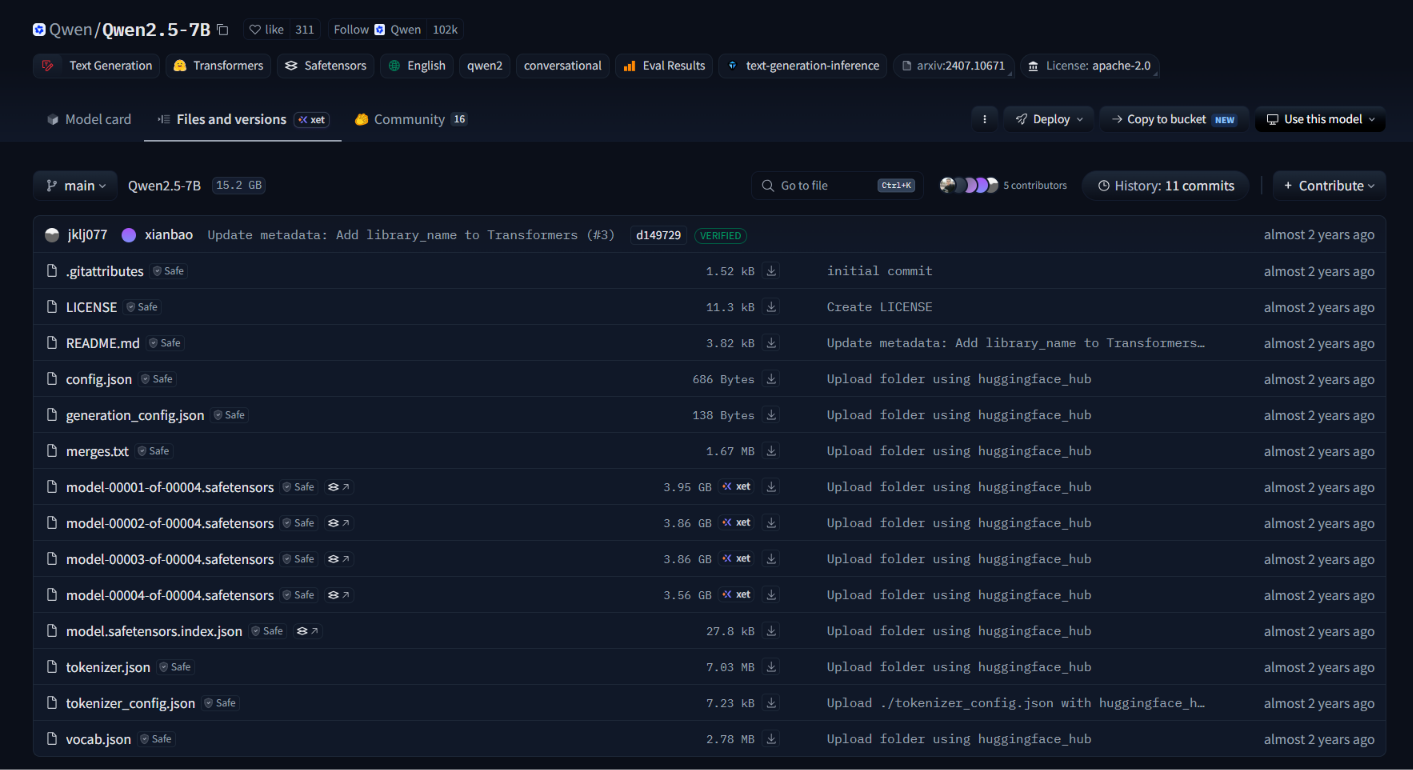
\includegraphics[width=\linewidth, height=0.44\textheight, keepaspectratio]{figures/case_sharded_weights_qwen.png}}}
            \end{center}
            \vspace{-0.2cm}
            \begin{infobox}[{\faSearch \ Sharded Weights (4 Mảnh)}]
                \tiny
                Model chia thành \texttt{00001} $\to$ \texttt{00004.safetensors} kèm \texttt{index.json}. Engine tự động gom nhóm để tính \texttt{weight\_set\_sha256}.
            \end{infobox}
        \end{column}
        \hfill
        \begin{column}{0.485\textwidth}
            \textbf{\textcolor{myaccent}{\faLayerGroup \ 1 Repo Đa Nhóm Weights (\texttt{LLaMA-3 GGUF})}}\\[3pt]
            \begin{center}
                {\setlength{\fboxsep}{1pt}\fcolorbox{myaccent!40}{white}{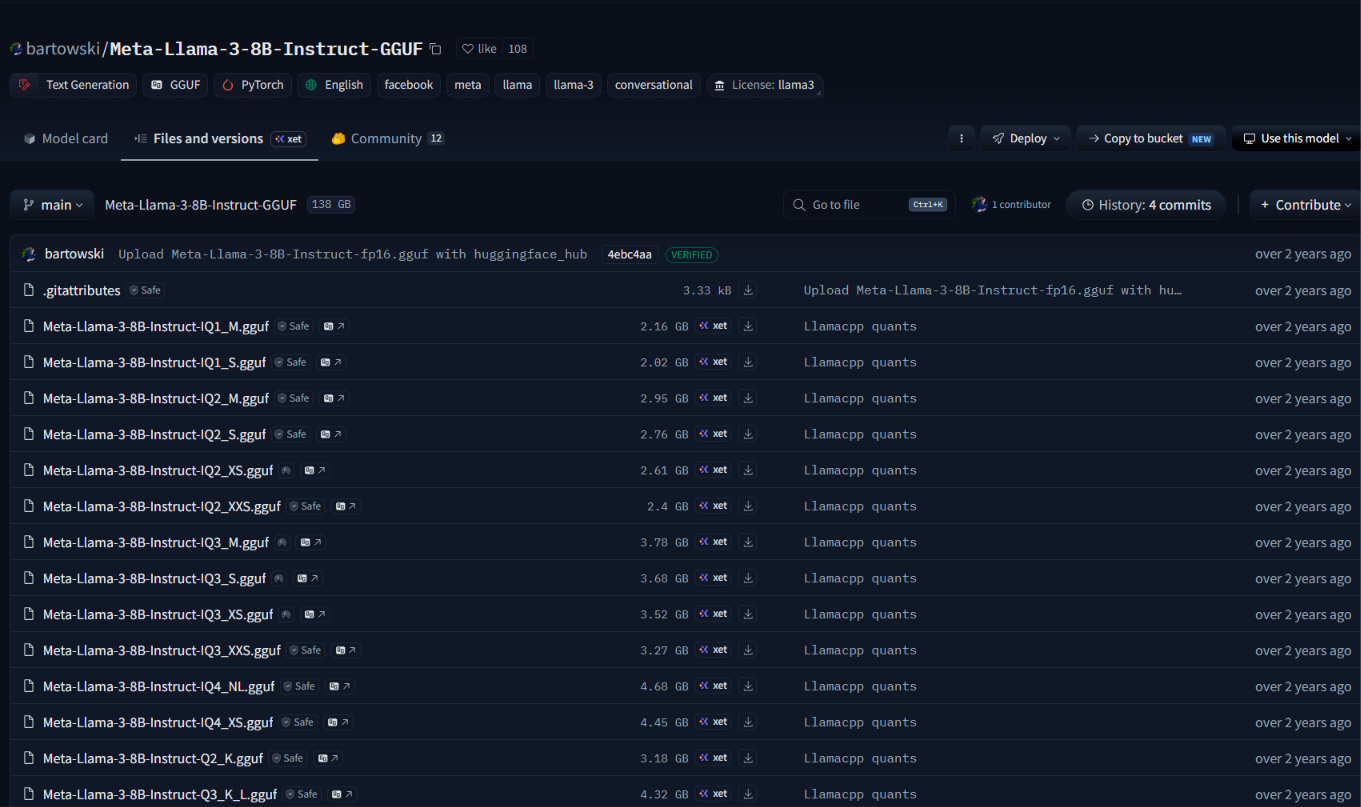
\includegraphics[width=\linewidth, height=0.44\textheight, keepaspectratio]{figures/case_multigroup_gguf_llama3.png}}}
            \end{center}
            \vspace{-0.2cm}
            \begin{infobox}[{\faShield* \ Multi-Group Withholding}]
                \tiny
                Chứa $>15$ phiên bản quant (\texttt{IQ1}, \texttt{IQ2}, \texttt{IQ4}). Engine kích hoạt withholding tại root để ngăn rò rỉ metadata sai lệch.
            \end{infobox}
        \end{column}
    \end{columns}
\end{frame}

\begin{frame}{Thực Tế Cấu Trúc Repo: Single Model \& Đa Định Dạng Weights}
    \begin{columns}[onlytextwidth, T]
        \begin{column}{0.485\textwidth}
            \textbf{\textcolor{mygreen}{\faCube \ 1 Model -- 1 Repo Chuẩn Mực (\texttt{CLIP})}}\\[3pt]
            \begin{center}
                {\setlength{\fboxsep}{1pt}\fcolorbox{mygreen!40}{white}{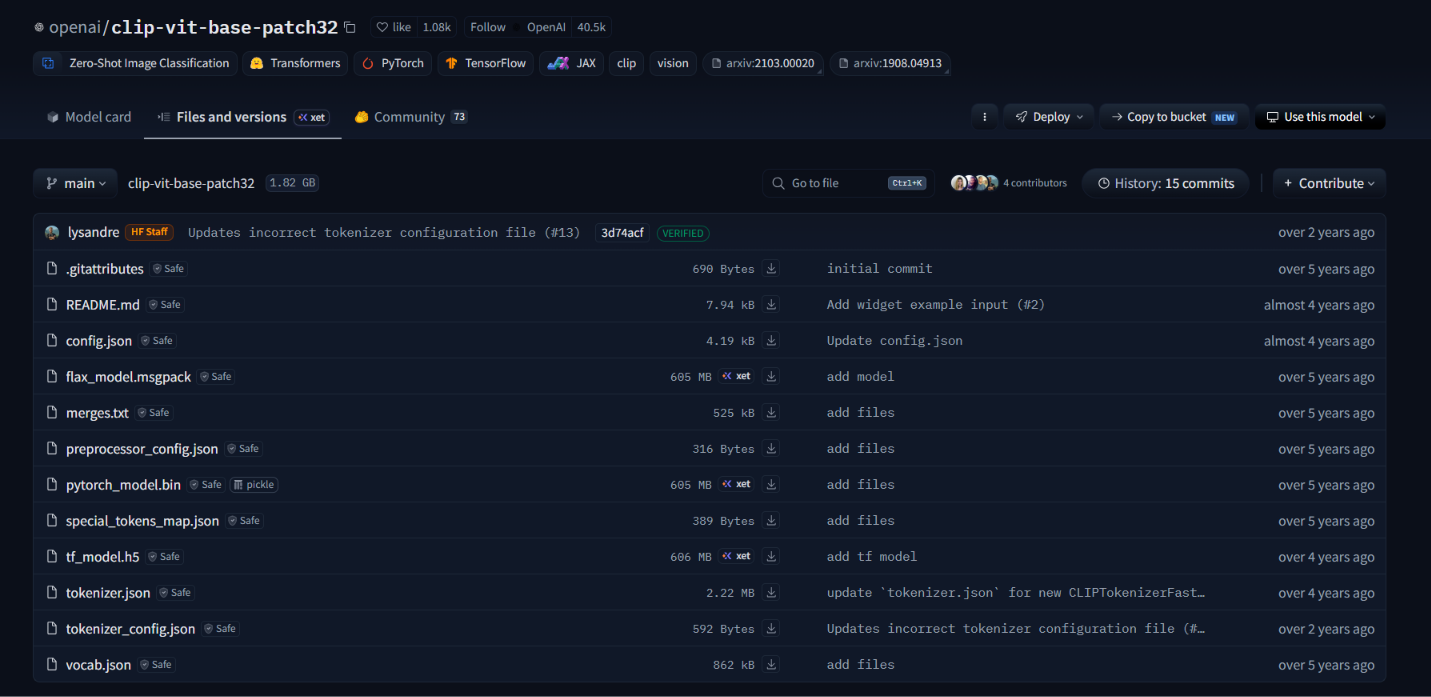
\includegraphics[width=\linewidth, height=0.44\textheight, keepaspectratio]{figures/case_single_model_clip.png}}}
            \end{center}
            \vspace{-0.2cm}
            \begin{infobox}[{\faCheckCircle \ Ánh Xạ 1--1 Tối Giản}]
                \tiny
                Chỉ chứa 1 model weights duy nhất kèm cấu hình. Ánh xạ trực tiếp $1-1$ với component trong tài liệu CycloneDX 1.6 ML-BOM.
            \end{infobox}
        \end{column}
        \hfill
        \begin{column}{0.485\textwidth}
            \textbf{\textcolor{mypurple}{\faBoxes \ 1 Repo Đa Định Dạng (\texttt{MiniLM})}}\\[3pt]
            \begin{center}
                {\setlength{\fboxsep}{1pt}\fcolorbox{mypurple!40}{white}{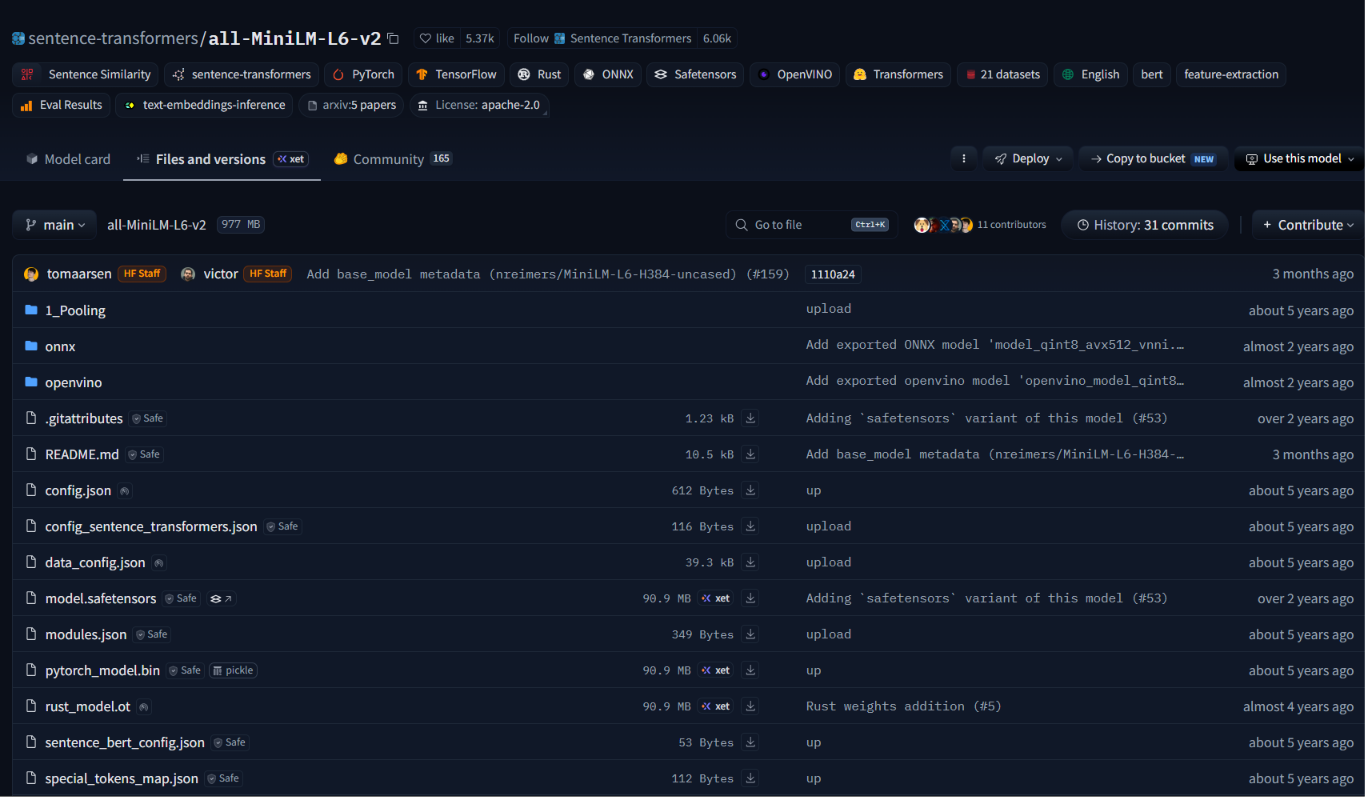
\includegraphics[width=\linewidth, height=0.44\textheight, keepaspectratio]{figures/case_multiformat_minilm.png}}}
            \end{center}
            \vspace{-0.2cm}
            \begin{infobox}[{\faCodeBranch \ Song Song Safetensors -- Bin -- ONNX}]
                \tiny
                Cùng 1 model nhưng có cả \texttt{.safetensors}, \texttt{.bin}, \texttt{onnx/}, \texttt{openvino/}. Engine gom nhóm theo kiến trúc tương đương.
            \end{infobox}
        \end{column}
    \end{columns}
\end{frame}

\begin{frame}{Thực Tế Hugging Face: Bùng Nổ Biến Thể \& Nhầm Lẫn Định Danh}
    \begin{columns}[onlytextwidth, T]
        \begin{column}{0.58\textwidth}
            \textbf{\textcolor{myalert}{\faSearch \ 6.899 Repos Phái Sinh Khớp \texttt{bert-base-uncased}}}\\[3pt]
            \begin{center}
                {\setlength{\fboxsep}{1pt}\fcolorbox{myalert!40}{white}{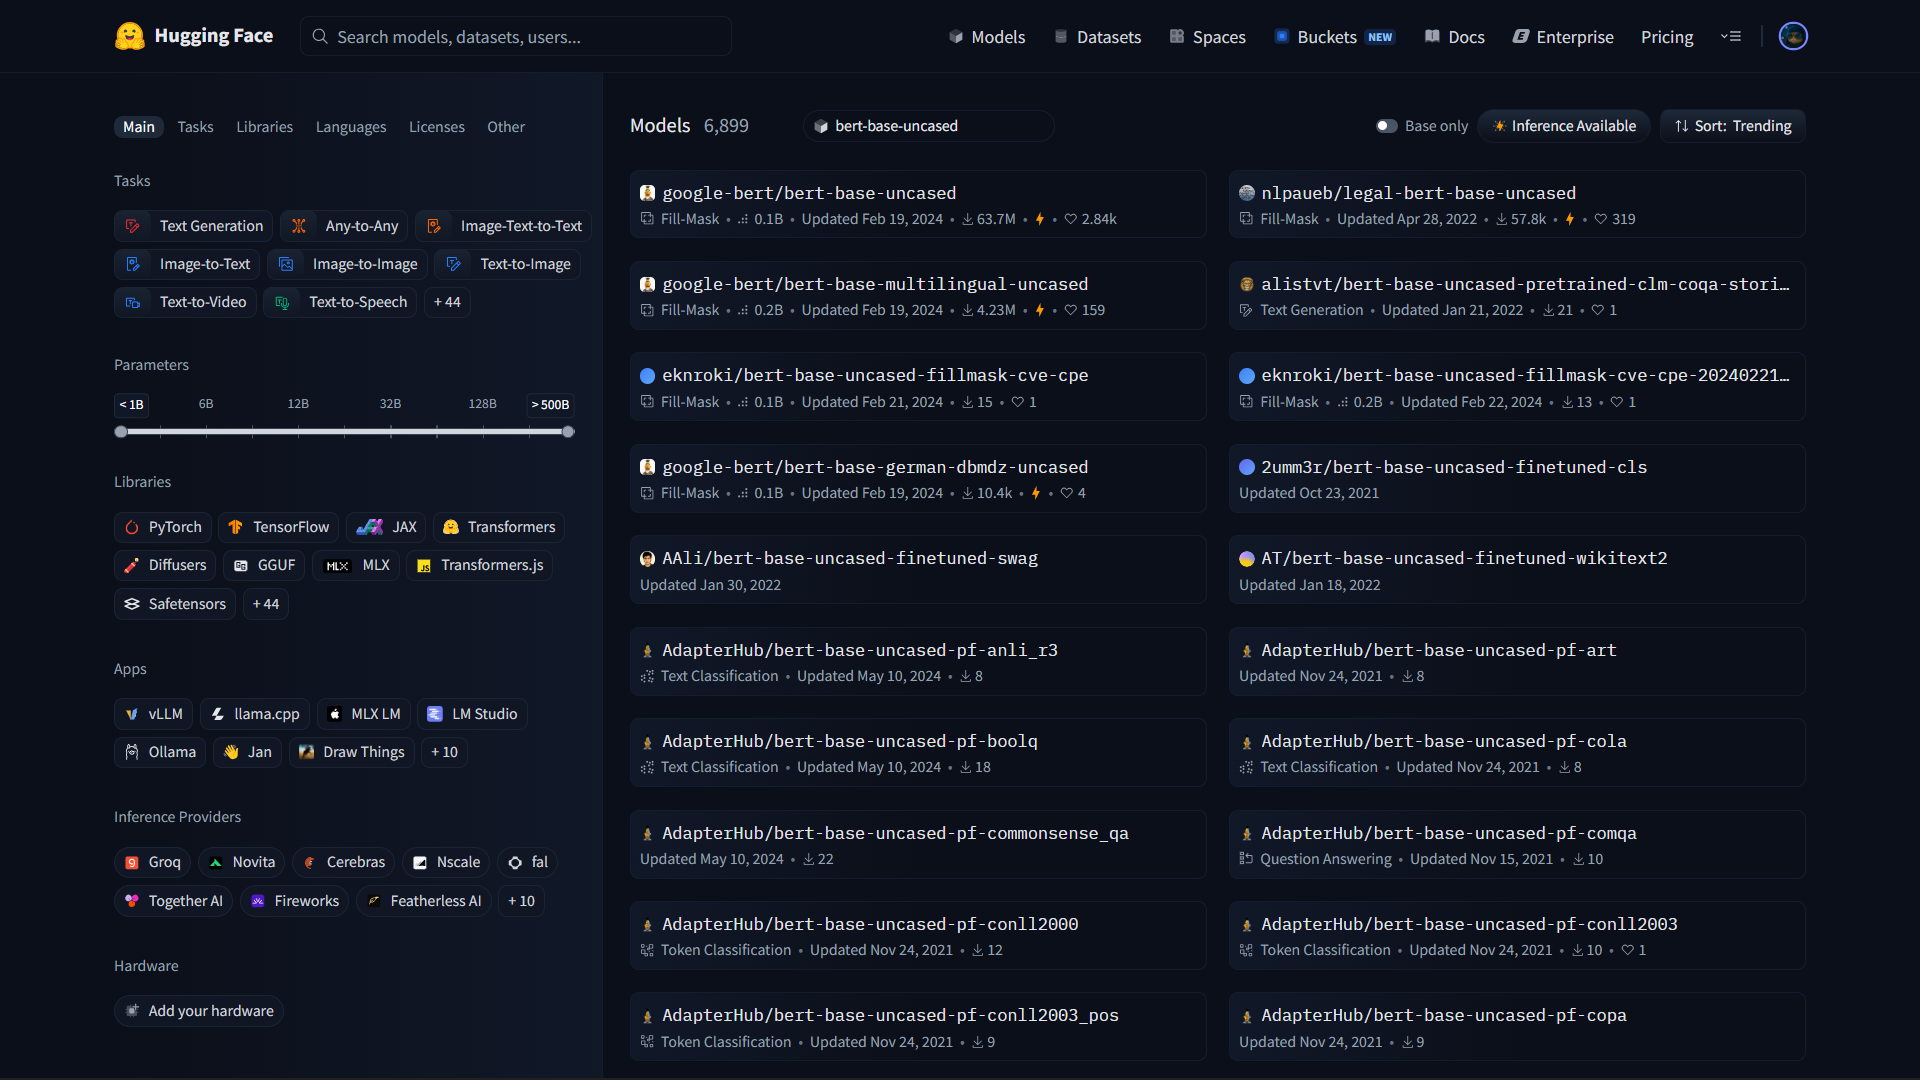
\includegraphics[width=\linewidth, height=0.60\textheight, keepaspectratio]{figures/case_multirepo_fanout_bert.png}}}
            \end{center}
        \end{column}
        \hfill
        \begin{column}{0.40\textwidth}
            \begin{warnbox}[{\faExclamationTriangle \ Bùng Nổ Mô Hình Phái Sinh}]
                \scriptsize
                6.899 kết quả cùng tên gốc \texttt{bert} nhưng:
                \begin{itemize}
                    \tiny
                    \item \textbf{Mirror / Clone}: Trùng 100\% hash weights gốc.
                    \item \textbf{File phụ}: \texttt{tokenizer.json} dùng chung ở 1.037 repos.
                    \item \textbf{Finetune}: Đã sửa weights, mang hash mới.
                \end{itemize}
            \end{warnbox}
            \vspace{-0.1cm}
            \begin{infobox}[{\faShield* \ Giải Pháp: Bắt Buộc Dùng Hash}]
                \scriptsize
                \begin{itemize}
                    \tiny
                    \item \textbf{Băm nhị phân}: Phân định rạch ròi Exact match vs Finetune (không đoán mò theo tên web).
                    \item \textbf{Candidates list}: Lưu toàn bộ repo trùng hash để kiểm toán bản quyền minh bạch.
                \end{itemize}
            \end{infobox}
        \end{column}
    \end{columns}
\end{frame}

\begin{frame}{Kiến Trúc SQLite 2 Tầng: Tách Biệt Raw Data \& Cache}
    \begin{figure}
        \centering
        \resizebox{0.96\textwidth}{!}{
        \begin{tikzpicture}[auto, >=Latex, font=\footnotesize]
            % L1 Node
            \node[draw=myprimary, fill=myprimary!8, rounded corners=4pt, text width=3.6cm, minimum height=2.5cm, align=center, drop shadow] (L1) at (0,0) {
                \textbf{\textcolor{myprimary}{\normalsize LAYER 1: Raw Store}}\\[3pt]
                \texttt{\textbf{aibom\_raw.sqlite}} (~4 GB)\\[3pt]
                \scriptsize Lưu raw JSON phản hồi HTTP, headers, ETag\\[3pt]
                \textbf{\textcolor{myalert}{\scriptsize Internal Only — 0 Phân Phối}}
            };
            
            % L2 Node
            \node[draw=myaccent, fill=myaccent!8, rounded corners=4pt, text width=4.0cm, minimum height=2.5cm, align=center, drop shadow] (L2) at (6.8,0) {
                \textbf{\textcolor{myaccent}{\normalsize LAYER 2: \mbox{Indexed Cache}}}\\[3pt]
                \texttt{\textbf{aibom.sqlite}} (~912 MB)\\[3pt]
                \scriptsize Chuẩn hóa 40 cột, index SHA-256\\[1pt]
                \scriptsize Allowlist 17 keys (18 KB/model)\\[3pt]
                \textbf{\textcolor{mygreen}{\scriptsize Phân Phối Kèm Engine}}
            };
            
            % L3 Node
            \node[draw=mygreen, fill=mygreen!8, rounded corners=4pt, text width=3.4cm, minimum height=2.5cm, align=center, drop shadow] (L3) at (13.4,0) {
                \textbf{\textcolor{mygreen}{\normalsize LAYER 3: Scanner}}\\[3pt]
                \texttt{\textbf{aibom-core}} (Rust)\\[3pt]
                \scriptsize Quét binary local, sniff header\\[3pt]
                \textbf{\textcolor{myprimary}{\scriptsize 100\% Offline (0 Mạng)}}
            };
            
            % Wide arrows with centered labels
            \draw[->, line width=1.4pt, myprimary] (L1.east) -- (L2.west);
            \node[above=4pt, align=center, font=\scriptsize\bfseries, text=myprimary] at ($(L1.east)!0.5!(L2.west)$) {Offline Replay\\[2pt]\fontsize{6.5}{7.5}\selectfont (0 request mạng)};
            
            \draw[->, line width=1.4pt, myaccent] (L2.east) -- (L3.west);
            \node[above=4pt, align=center, font=\scriptsize\bfseries, text=myaccent] at ($(L2.east)!0.5!(L3.west)$) {Read-Only\\[2pt]\fontsize{6.5}{7.5}\selectfont (Query $<1\text{ms}$)};
        \end{tikzpicture}
        }
    \end{figure}
    \vspace{-0.2cm}
    \begin{infobox}[{\faLightbulb \hspace{2pt} Lợi Ích Của Thiết Kế 2 Tầng}]
        \scriptsize
        \begin{itemize}
            \item \textbf{Gọn nhẹ}: DB phân phối kèm scanner chỉ nặng ~912 MB (~18 KB/model).
            \item \textbf{Offline Replayability}: Khi cập nhật quy tắc chuẩn hóa, rebuild L2 từ L1 trong vài phút, 0 cần thu thập lại qua mạng.
        \end{itemize}
    \end{infobox}
\end{frame}

\begin{frame}{Sơ Đồ Trực Quan: Cơ Chế Offline Replayability (Layer 1 $\to$ Layer 2)}
    \begin{center}
    \resizebox{0.96\textwidth}{!}{
    \begin{tikzpicture}[auto, >=Latex, font=\scriptsize]
        % Top comparison: 1-tier
        \node[draw=myalert, fill=myalert!8, rounded corners=4pt, text width=2.2cm, minimum height=1.5cm, align=center] (api1) at (-0.9, 1.45) {
            \textbf{\faGlobe \ Web API}\\[2pt]
            \tiny Hugging Face Hub
        };
        \node[draw=myalert, fill=myalert!8, rounded corners=4pt, text width=2.8cm, minimum height=1.5cm, align=center] (db1) at (10.5, 1.45) {
            \textbf{\faDatabase \ Ingestion Đơn Tầng}\\[2pt]
            \tiny SQLite Scanner Cục Bộ
        };
        \draw[->, line width=1.3pt, myalert] (api1.east) -- 
            node[above=3pt, font=\tiny\bfseries, text=myalert, align=center] {Thu Thập Trực Tiếp (6--8 tiếng)} 
            node[below=3pt, font=\tiny, text=black!70, align=center] {Thay đổi quy tắc chuẩn hóa $\to$ Bắt buộc nạp lại từ đầu qua mạng!} (db1.west);
        \node[draw=myalert, fill=myalert!20, circle, inner sep=2.5pt] at (12.5, 1.45) {\normalsize \textcolor{myalert}{\faTimes}};

        % Separator
        \draw[dashed, line width=0.8pt, black!25] (-2.2, 0.3) -- (13.2, 0.3);

        % Bottom: 2-tier architecture
        \node[draw=mygreen, fill=mygreen!8, rounded corners=4pt, text width=2.2cm, minimum height=1.8cm, align=center] (api2) at (-0.9, -1.0) {
            \textbf{\faGlobe \ Web API}\\[2pt]
            \tiny Hugging Face Hub
        };
        \node[draw=myprimary, fill=myprimary!10, rounded corners=4pt, text width=2.6cm, minimum height=1.8cm, align=center, drop shadow] (l1) at (4.2, -1.0) {
            \textbf{\faArchive \ Layer 1: Raw}\\[2pt]
            \texttt{\textbf{aibom\_raw.sqlite}}\\[1pt]
            \tiny ($\approx$4 GB) $\bullet$ Lưu 1 lần\\[2pt]
            \tiny Raw JSON Ingestion
        };
        \node[draw=myaccent, fill=myaccent!10, rounded corners=4pt, text width=2.8cm, minimum height=1.8cm, align=center, drop shadow] (l2) at (10.5, -1.0) {
            \textbf{\faDatabase \ Layer 2: Cache}\\[2pt]
            \texttt{\textbf{aibom.sqlite}}\\[1pt]
            \tiny ($\approx$912 MB) $\bullet$ 17 keys\\[2pt]
            \tiny Indexed Cache Phân Phối
        };
        
        \draw[->, line width=1.3pt, mygreen] (api2.east) -- 
            node[above=3pt, font=\tiny\bfseries, text=mygreen, align=center] {Ingestion 1 Lần} (l1.west);
        \draw[->, line width=1.4pt, myaccent] (l1.east) -- 
            node[above=3pt, font=\tiny\bfseries, text=myaccent, align=center] {Offline Replay (Rust)} 
            node[below=3pt, font=\tiny\bfseries, text=myprimary, align=center] {Rebuild $<5$ phút (0 mạng)} (l2.west);
        \node[draw=mygreen, fill=mygreen!20, circle, inner sep=2.5pt] at (12.5, -1.0) {\normalsize \textcolor{mygreen}{\faCheck}};
    \end{tikzpicture}
    }
    \end{center}
    \vspace{-0.2cm}
    \begin{infobox}[{\faShield* \hspace{2pt} Ý Nghĩa Kiến Trúc}]
        \scriptsize
        Tách biệt hoàn toàn tầng lưu trữ nguyên thủy (Raw Ingestion) và tầng lập chỉ mục (Clean Projection). Giúp kỹ sư thử nghiệm hàng chục bộ quy tắc chuẩn hóa mà không gây nghẽn mạng hay bị khóa API.
    \end{infobox}
\end{frame}

\begin{frame}{Sơ Đồ Kiến Trúc Toàn Hệ Thống (3-Layer Data Flow)}
    \begin{center}
    \resizebox{0.96\textwidth}{!}{
    \begin{tikzpicture}[auto, >=Latex, font=\scriptsize]
        % ----------------------------------------------------
        % LAYER 1 Container
        % ----------------------------------------------------
        \node[draw=myprimary!60, fill=myprimary!5, rounded corners=6pt, dashed, line width=0.8pt, 
              minimum width=5.6cm, minimum height=2.6cm] (l1_box) at (1.8, 2.3) {};
        \node[anchor=north west, font=\fontsize{6.5}{7.5}\selectfont\bfseries, text=myprimary] at (l1_box.north west) {
            \hspace{3pt} \faArchive \ LAYER 1: Ingestion \& Harvest (Internal)
        };
        
        \node[draw=myprimary, fill=white, rounded corners=3pt, text width=1.8cm, align=center] (hf) at (0.2, 2.15) {
            \textbf{\faGlobe \ HF Hub}\\[1pt]
            \tiny API \& Git
        };
        \node[draw=myprimary, fill=myprimary!12, rounded corners=3pt, text width=2.0cm, align=center, drop shadow] (l1) at (3.6, 2.15) {
            \textbf{\faDatabase \ Raw Store}\\[1pt]
            \texttt{\tiny aibom\_raw.sqlite}\\[1pt]
            \tiny ($\approx$4 GB)
        };
        \draw[->, line width=1.2pt, myprimary] (hf.east) -- node[above=2pt, font=\fontsize{6}{7}\selectfont\bfseries, text=myprimary] {Worker} (l1.west);

        % ----------------------------------------------------
        % LAYER 2 Container
        % ----------------------------------------------------
        \node[draw=myaccent!70, fill=myaccent!5, rounded corners=6pt, line width=0.8pt, 
              minimum width=10.4cm, minimum height=2.6cm] (l2_box) at (13.6, 2.3) {};
        \node[anchor=north west, font=\fontsize{6.5}{7.5}\selectfont\bfseries, text=myaccent] at (l2_box.north west) {
            \hspace{3pt} \faDatabase \ LAYER 2: Indexed Cache (\texttt{aibom.sqlite} $\approx$912 MB $\bullet$ Phân Phối Kèm Scanner)
        };

        % Rebuild arrow from L1 directly to l2_main
        \node[draw=myaccent, fill=myaccent!12, rounded corners=3pt, text width=2.4cm, align=center, drop shadow] (l2_main) at (10.0, 2.15) {
            \textbf{\faSearch \ Cache DB}\\[1pt]
            \texttt{\tiny aibom.sqlite}\\[1pt]
            \tiny Index B-Tree
        };
        
        \draw[->, line width=1.4pt, myaccent] (l1.east) -- 
            node[above=2pt, font=\fontsize{6}{7}\selectfont\bfseries, text=myaccent, fill=white, inner sep=1.5pt, rounded corners=2pt, align=center] {Offline Replay (Rust)} 
            node[below=2pt, font=\fontsize{5.5}{6.5}\selectfont\bfseries, text=myprimary, fill=white, inner sep=1.5pt, rounded corners=2pt, align=center] {Rebuild (0 mạng)} (l2_main.west);

        % Tables inside Layer 2
        \node[draw=myaccent!80, fill=white, rounded corners=2pt, text width=2.5cm, align=center] (t_model) at (13.7, 2.6) {
            \textbf{\texttt{\tiny model}}\\[-1pt]
            \fontsize{5}{6}\selectfont 40 cột DDL chuẩn
        };
        \node[draw=myaccent!80, fill=white, rounded corners=2pt, text width=2.5cm, align=center] (t_file) at (17.0, 2.6) {
            \textbf{\texttt{\tiny model\_file}}\\[-1pt]
            \fontsize{5}{6}\selectfont Hashes, roles, sizes
        };
        \node[draw=myaccent!80, fill=white, rounded corners=2pt, text width=2.5cm, align=center] (t_ws) at (13.7, 1.65) {
            \textbf{\texttt{\tiny weight\_set}}\\[-1pt]
            \fontsize{5}{6}\selectfont Nhóm weights sharded
        };
        \node[draw=myaccent!80, fill=white, rounded corners=2pt, text width=2.5cm, align=center] (t_fts) at (17.0, 1.65) {
            \textbf{\texttt{\tiny fts\_model}}\\[-1pt]
            \fontsize{5}{6}\selectfont FTS5 full-text search
        };

        \draw[-, line width=0.6pt, myaccent!60] (l2_main.east) -- (t_model.west);
        \draw[-, line width=0.6pt, myaccent!60] (l2_main.east) -- (t_ws.west);

        % ----------------------------------------------------
        % LAYER 3 Container (Offline Scanner Engine)
        % ----------------------------------------------------
        \node[draw=mygreen!80, fill=mygreen!5, rounded corners=6pt, line width=0.9pt, 
              minimum width=19.8cm, minimum height=2.6cm] (l3_box) at (9.2, -1.0) {};
        \node[anchor=north west, font=\fontsize{6.5}{7.5}\selectfont\bfseries, text=mygreen] at (l3_box.north west) {
            \hspace{3pt} \faCogs \ LAYER 3: Offline Scanner Engine (\texttt{aibom-core} Rust $\bullet$ 100\% Zero-Network)
        };

        \node[draw=mygreen, fill=white, rounded corners=3pt, text width=2.1cm, align=center] (target) at (0.2, -1.15) {
            \textbf{\faFolderOpen \ Artifact}\\[1pt]
            \tiny File / Thư mục
        };
        \node[draw=mygreen, fill=white, rounded corners=3pt, text width=2.1cm, align=center] (sniff) at (3.5, -1.15) {
            \textbf{\faBolt \ Sniffer}\\[1pt]
            \tiny Header $<5\text{ms}$
        };
        \node[draw=mygreen, fill=white, rounded corners=3pt, text width=2.5cm, align=center] (group) at (6.8, -1.15) {
            \textbf{\faFilter \ Phân Loại File}\\[1pt]
            \tiny Gom nhóm weights
        };
        \node[draw=myprimary, fill=myprimary!10, rounded corners=3pt, text width=2.6cm, align=center, drop shadow] (resolve) at (10.0, -1.15) {
            \textbf{\faSearch \ Match Resolver}\\[1pt]
            \tiny Exact SHA $\to$ Heuristic
        };
        \node[draw=mygreen, fill=white, rounded corners=3pt, text width=2.3cm, align=center] (enrich) at (13.5, -1.15) {
            \textbf{\faBalanceScale \ Hòa Giải}\\[1pt]
            \tiny Lọc floor, merge
        };
        \node[draw=mygreen, fill=mygreen!15, rounded corners=3pt, text width=2.3cm, align=center, drop shadow] (out) at (16.9, -1.15) {
            \textbf{\faFileCode \ Output BOM}\\[1pt]
            \tiny CycloneDX 1.6
        };

        % Layer 3 intra-pipeline arrows with generous spacing
        \draw[->, line width=1.3pt, mygreen] (target.east) -- (sniff.west);
        \draw[->, line width=1.3pt, mygreen] (sniff.east) -- (group.west);
        \draw[->, line width=1.3pt, mygreen] (group.east) -- (resolve.west);
        \draw[->, line width=1.3pt, mygreen] (resolve.east) -- (enrich.west);
        \draw[->, line width=1.3pt, mygreen] (enrich.east) -- (out.west);

        % Cross-layer connection: Layer 2 Cache to Layer 3 Match Resolver (PERFECTLY VERTICAL)
        \draw[->, line width=1.4pt, dashed, myaccent] (l2_main.south) -- 
            node[pos=0.22, right=4pt, font=\fontsize{5.5}{6.5}\selectfont\bfseries, text=myaccent, fill=white, inner sep=2pt, rounded corners=2pt, align=left] {Read-Only Query\\[1pt]\tiny($<1\text{ms}$)} (resolve.north);
    \end{tikzpicture}
    }
    \end{center}
    \vspace{-0.2cm}
    \begin{infobox}[{\faShield* \hspace{2pt} Kiến Trúc 3 Tầng: Thu Thập -- Bộ Đệm -- Động Cơ Quét}]
        \scriptsize
        Layer 1 thu thập raw JSON nội bộ $\to$ Layer 2 lập chỉ mục siêu nhẹ ($\approx$18 KB/model) phân phối kèm scanner $\to$ Layer 3 quét nhị phân ngoại tuyến 100\% không cần kết nối mạng.
    \end{infobox}
\end{frame}

\begin{frame}{Bộ Lọc 17 Trường Quan Trọng Từ Model Card (Allowlist)}
    \begin{columns}[onlytextwidth, T]
        \begin{column}{0.48\textwidth}
            \begin{infobox}[{\faListUl \hspace{2pt} 17 Trường Cần Thiết Được Giữ Lại}]
                \scriptsize
                Chỉ giữ đúng 17 trường có giá trị kiểm toán:
                \begin{enumerate}
                    \tiny
                    \item \texttt{license} \hfill 10. \texttt{model\_name}
                    \item \texttt{library\_name} \hfill 11. \texttt{license\_name}
                    \item \texttt{pipeline\_tag} \hfill 12. \texttt{license\_link}
                    \item \texttt{tags} \hfill 13. \texttt{widget}
                    \item \texttt{datasets} \hfill 14. \texttt{co2\_eq\_emissions}
                    \item \texttt{metrics} \hfill 15. \texttt{fine\_tuned\_from}
                    \item \texttt{base\_model} \hfill 16. \texttt{thumbnail}
                    \item \texttt{language} \hfill 17. \texttt{model\_type}
                    \item \texttt{inference}
                \end{enumerate}
            \end{infobox}
        \end{column}
        \hfill
        \begin{column}{0.48\textwidth}
            \begin{successbox}[{\faCompress \hspace{2pt} Hiệu Quả Nén Dữ Liệu}]
                \scriptsize
                \begin{itemize}
                    \item Loại bỏ văn bản phi cấu trúc dư thừa $\to$ dung lượng nén đạt \textbf{18.0 KB / model}.
                    \item Toàn bộ 50.000 models lưu gọn trong \textbf{~912 MB SQLite}.
                \end{itemize}
            \end{successbox}
        \end{column}
    \end{columns}
\end{frame}

\begin{frame}[fragile]{Bảng Model \& Xử Lý Model Khai Báo License "Other"}
    \begin{lstlisting}[language=sql, basicstyle=\ttfamily\fontsize{5.5}{6.5}\selectfont]
CREATE TABLE model (
    repo_id TEXT PRIMARY KEY, author TEXT, model_name TEXT, sha TEXT,
    last_modified TEXT, private INTEGER, gated INTEGER, disabled INTEGER,
    pipeline_tag TEXT, library_name TEXT, model_type TEXT, model_architecture TEXT,
    license_spdx TEXT,
    license_name TEXT, -- Luu ten license goc khi khai bao "other"
    license_link TEXT, -- Luu link dieu khoan license goc
    downloads INTEGER, likes INTEGER, created_at TEXT,
    config_json TEXT, card_data_json TEXT, card_text_sha256 TEXT,
    weight_set_count INTEGER, weight_file_count INTEGER, total_weight_bytes INTEGER
    -- Tong cong 40 cot chuan hoa
);
    \end{lstlisting}
    \vspace{-0.1cm}
    \begin{successbox}[{\faCheck \hspace{2pt} Chuẩn Hóa 70.0\% Model Khai Báo License "Other"}]
        \scriptsize
        Tách riêng 2 cột \texttt{license\_name} \& \texttt{license\_link} $\to$ chuẩn hóa \textbf{3,466 / 4,950 models} khai \texttt{other} (đạt 70.0\%).
    \end{successbox}
\end{frame}

\begin{frame}[fragile]{Bảng File, Weight Set \& Ánh Xạ FileRole}
    \begin{lstlisting}[language=sql, basicstyle=\ttfamily\fontsize{5.5}{6.5}\selectfont]
CREATE TABLE model_file (
    repo_id TEXT, path TEXT, size_bytes INTEGER, sha256 TEXT, lfs_sha256 TEXT,
    role TEXT, -- weight | config | tokenizer | license | doc | other (DDL)
    PRIMARY KEY (repo_id, path)
);
CREATE TABLE weight_set (
    weight_set_sha256 TEXT PRIMARY KEY, -- Hash tong hop cua weight group
    repo_id TEXT, member_count INTEGER, total_bytes INTEGER
);
    \end{lstlisting}
    \vspace{-0.1cm}
    \begin{infobox}[{\faDatabase \hspace{2pt} Ánh Xạ 6 Role DDL Thô $\to$ 5 Cấp FileRole Trong Scanner}]
        \scriptsize
        \begin{itemize}
            \item \textbf{DB DDL (6 role thô)}: \texttt{weight}, \texttt{config}, \texttt{tokenizer}, \texttt{license}, \texttt{doc}, \texttt{other}.
            \item \textbf{Scanner Engine (5 FileRole)}: \texttt{Weight} (measured), \texttt{Auxiliary} (khóa trần heuristic cho config/tokenizer/license/doc), \texttt{Media}, \texttt{Archive}, \texttt{Other}.
        \end{itemize}
    \end{infobox}
\end{frame}

\begin{frame}{Sơ Đồ Thực Thể - Quan Hệ CSDL Cache L2 (\texttt{aibom.sqlite})}
    \begin{center}
    \resizebox{0.96\textwidth}{!}{
    \begin{tikzpicture}[auto, >=Latex, font=\scriptsize]
        % Table 1: model (Central Table)
        \node[draw=myprimary, fill=myprimary!8, rounded corners=3pt, text width=3.8cm, align=left, drop shadow] (model) at (0, 0) {
            \textbf{\faTable \ Bảng \texttt{model}}\\[2pt]
            \tiny \textbf{\textcolor{myalert}{\faKey \ repo\_id}} \texttt{TEXT PRIMARY KEY}\\
            \tiny $\bullet$ \texttt{author}, \texttt{model\_name}, \texttt{sha}\\
            \tiny $\bullet$ \texttt{pipeline\_tag}, \texttt{library\_name}\\
            \tiny $\bullet$ \texttt{license\_spdx}, \texttt{license\_name}\\
            \tiny $\bullet$ \texttt{config\_json}, \texttt{card\_data\_json}\\
            \tiny $\bullet$ \dots (40 cột chuẩn hóa)\\
            \vspace{1pt}
            \centering \tiny \textit{49,992 models đại diện}
        };

        % Table 2: model_file (1-N from model)
        \node[draw=myaccent, fill=myaccent!8, rounded corners=3pt, text width=3.8cm, align=left, drop shadow] (file) at (5.6, 1.55) {
            \textbf{\faTable \ Bảng \texttt{model\_file}}\\[2pt]
            \tiny \textbf{\textcolor{myalert}{\faKey \ (repo\_id, path)}} \texttt{PRIMARY KEY}\\
            \tiny $\bullet$ \texttt{repo\_id} (\textbf{\textcolor{myprimary}{FK $\to$ model}})\\
            \tiny $\bullet$ \textbf{\textcolor{mygreen}{\faSearch \ sha256}} \texttt{TEXT} \textbf{(B-Tree Index)}\\
            \tiny $\bullet$ \texttt{lfs\_sha256}, \texttt{size\_bytes}\\
            \tiny $\bullet$ \texttt{role} (\textit{weight, config, doc...})\\
            \vspace{1pt}
            \centering \tiny \textit{798,682 file hashes (Tra cứu $<1$ms)}
        };

        % Table 3: weight_set (1-N from model)
        \node[draw=myorange, fill=myorange!8, rounded corners=3pt, text width=3.8cm, align=left, drop shadow] (ws) at (5.6, -1.55) {
            \textbf{\faTable \ Bảng \texttt{weight\_set}}\\[2pt]
            \tiny \textbf{\textcolor{myalert}{\faKey \ weight\_set\_sha256}} \texttt{PK (Index)}\\
            \tiny $\bullet$ \texttt{repo\_id} (\textbf{\textcolor{myprimary}{FK $\to$ model}})\\
            \tiny $\bullet$ \texttt{member\_count}, \texttt{total\_bytes}\\
            \vspace{1pt}
            \centering \tiny \textit{47,854 chữ ký cụm Shards}
        };

        % Table 4: harvest_gap (1-N from model)
        \node[draw=mypurple, fill=mypurple!8, rounded corners=3pt, text width=3.2cm, align=left, drop shadow] (gap) at (10.6, 0) {
            \textbf{\faTable \ Bảng \texttt{harvest\_gap}}\\[2pt]
            \tiny \textbf{\textcolor{myalert}{\faKey \ (repo\_id, field, ...)}}\\
            \tiny $\bullet$ \texttt{repo\_id} (\textbf{\textcolor{myprimary}{FK $\to$ model}})\\
            \tiny $\bullet$ \texttt{field}, \texttt{provider}\\
            \tiny $\bullet$ \texttt{pointer NOT NULL DEFAULT ''}\\
            \vspace{1pt}
            \centering \tiny \textit{Audit thiếu sót dữ liệu}
        };

        % Relationships
        \draw[->, line width=1.2pt, myprimary] (model.east) -- ++(0.4,0) |- (file.west) node[near start, above, font=\tiny\bfseries] {1 : N};
        \draw[->, line width=1.2pt, myprimary] (model.east) -- ++(0.4,0) |- (ws.west) node[near start, below, font=\tiny\bfseries] {1 : N};
        \draw[->, line width=1.2pt, myaccent] (model.east) -- (gap.west) node[pos=0.88, above, font=\tiny\bfseries] {1 : N};
    \end{tikzpicture}
    }
    \end{center}
    \vspace{-0.2cm}
    \begin{infobox}[{\faSearch \hspace{2pt} Tối Ưu Hóa Tốc Độ Tra Cứu (Zero-Scan Overhead)}]
        \scriptsize
        Chỉ mục B-Tree trên cột \texttt{sha256} và \texttt{weight\_set\_sha256} cho phép scanner tra cứu tức thì danh tính model và candidate repos trong \textbf{dưới 1ms}, hoàn toàn độc lập với kích thước cơ sở dữ liệu.
    \end{infobox}
\end{frame}

\begin{frame}[fragile]{Bảng Ghi Nhận Thiếu Sót (Gaps) \& Tối Ưu DB}
    \begin{columns}[onlytextwidth, T]
        \begin{column}{0.54\textwidth}
            \begin{lstlisting}[language=sql, basicstyle=\ttfamily\fontsize{5.5}{6.5}\selectfont]
CREATE TABLE harvest_gap (
    repo_id  TEXT NOT NULL,
    field    TEXT NOT NULL,
    provider TEXT NOT NULL,
    pointer  TEXT NOT NULL DEFAULT '', -- Tranh loi NULL cua SQLite
    PRIMARY KEY (repo_id, field, provider, pointer)
);
            \end{lstlisting}
            \begin{infobox}[{\faKey \hspace{2pt} Khóa Chính 4 Cột Tránh Lọt Bản Ghi Trùng}]
                \scriptsize
                SQLite coi \texttt{NULL != NULL} $\to$ dùng \texttt{pointer NOT NULL DEFAULT ''} để bảo đảm lọc trùng chính xác 100\%.
            \end{infobox}
        \end{column}
        \hfill
        \begin{column}{0.44\textwidth}
            \begin{successbox}[{\faSnowflake \hspace{2pt} Đóng Băng File SQLite Trước Khi Ship}]
                \scriptsize
                Lệnh tối ưu trước khi release:
                \begin{lstlisting}[language=sql, basicstyle=\ttfamily\fontsize{5}{6}\selectfont]
PRAGMA journal_mode = DELETE;
PRAGMA wal_autocheckpoint = 0;
VACUUM;
                \end{lstlisting}
                \begin{itemize}
                    \item 1 file duy nhất, read-only, không sinh file phụ \texttt{-wal}.
                \end{itemize}
            \end{successbox}
        \end{column}
    \end{columns}
\end{frame}

% ============================================================
% PHẦN 3: QUY TẮC ĐÁNH GIÁ ĐỘ TIN CẬY & XỬ LÝ XUNG ĐỘT
% ============================================================
\section{Quy Tắc Đánh Giá Độ Tin Cậy \& Xử Lý Xung Đột}

\begin{frame}{Sơ Đồ Luồng Thực Thi Runtime Của \texttt{aibom-core}}
    \begin{figure}
        \centering
        \resizebox{0.96\textwidth}{!}{
        \begin{tikzpicture}[auto, >=Latex, font=\scriptsize]
            % Target node
            \node[draw=myprimary, fill=myprimary!8, rounded corners, text width=2.4cm, align=center, drop shadow] (target) at (0, 2) {
                \textbf{\textcolor{myprimary}{Target Artifact}}\\[2pt]
                \tiny File / Directory local
            };
            
            % Step 1: dirscan & Gom nhóm weights
            \node[draw=myprimary, fill=myprimary!12, rounded corners, text width=3.0cm, align=center, drop shadow] (step1) at (3.8, 2) {
                \textbf{\textcolor{myprimary}{1. dirscan \& Gom Nhóm}}\\[2pt]
                \tiny \texttt{fileset.rs} · Phân loại FileRole\\Gom Shards, ONNX data
            };
            
            % Step 2: Phase 1 Sniffing
            \node[draw=myaccent, fill=myaccent!10, rounded corners, text width=3.4cm, align=center, drop shadow] (phase1) at (8.2, 3.2) {
                \textbf{\textcolor{myaccent}{Phase 1: Sniffer ($<5\text{ms}$)}}\\[2pt]
                \tiny \texttt{formats/*} · Header parser\\Tensor shapes, Pickle safe
            };
            
            % Step 3: Phase 2 Streaming Hash
            \node[draw=myorange, fill=myorange!10, rounded corners, text width=3.4cm, align=center, drop shadow] (phase2) at (8.2, 0.8) {
                \textbf{\textcolor{myorange}{Phase 2: Streaming Hash}}\\[2pt]
                \tiny \texttt{util.rs} · Chunking ($<50\text{MB}$ RAM)\\File SHA, \texttt{weight\_set\_sha256}
            };
            
            % Step 4: Query L2
            \node[draw=myprimary, fill=myprimary!8, rounded corners, text width=3.0cm, align=center, drop shadow] (step4) at (12.6, 0.8) {
                \textbf{\textcolor{myprimary}{4. Query Cache L2}}\\[2pt]
                \tiny \texttt{db.rs} · \texttt{aibom.sqlite}\\Tra cứu SHA $\to$ $N$ candidates
            };
            
            % Step 5: Policy Gate & Combinators
            \node[draw=mypurple, fill=mypurple!10, rounded corners, text width=3.8cm, align=center, drop shadow] (step5) at (12.6, 3.2) {
                \textbf{\textcolor{mypurple}{5. Policy \& Hòa Giải}}\\[2pt]
                \tiny \texttt{policy.rs}, \texttt{evidence.rs}\\Lọc Floor, \texttt{from\_claims}, Round-Robin
            };
            
            % Step 6: Output Emitter
            \node[draw=mygreen, fill=mygreen!12, rounded corners, text width=2.8cm, align=center, drop shadow] (step6) at (17.2, 2) {
                \textbf{\textcolor{mygreen}{6. Output Emitter}}\\[2pt]
                \tiny \texttt{cyclonedx.rs} · CycloneDX 1.6\\report/2 Envelope, Withholding
            };
            
            % Connecting lines
            \draw[->, line width=1.2pt, myprimary] (target) -- (step1);
            \draw[->, line width=1.2pt, myaccent] (step1.east) -- (phase1.west);
            \draw[->, line width=1.2pt, myorange] (step1.east) -- (phase2.west);
            \draw[->, line width=1.2pt, myorange] (phase2) -- (step4);
            \draw[->, line width=1.2pt, myprimary] (step4) -- (step5);
            \draw[->, line width=1.2pt, myaccent] (phase1) -- (step5);
            \draw[->, line width=1.2pt, mygreen] (step5.east) -- (step6);
        \end{tikzpicture}
        }
    \end{figure}
    \vspace{-0.2cm}
    \begin{infobox}[{{\faCogs \hspace{2pt} Quy Trình Thực Thi Khép Kín 100\% Offline}}]
        \scriptsize
        Dữ liệu di chuyển tuần tự qua 7 module Rust độc lập, không chia sẻ trạng thái toàn cục, bảo đảm tính tất định và an toàn bộ nhớ.
    \end{infobox}
\end{frame}

\begin{frame}{Hệ Thống 4 Cấp Evidence Class (Evidence Levels)}
    $$\text{\textbf{heuristic (0)}} < \text{\textbf{declared (1)}} < \text{\textbf{verified (2)}} < \text{\textbf{measured (3)}}$$
    
    \begin{table}
        \centering
        \scriptsize
        \renewcommand{\arraystretch}{1.05}
        \begin{tabular}{c l p{0.36\textwidth} p{0.36\textwidth}}
            \toprule
            \textbf{Cấp} & \textbf{Evidence Class} & \textbf{Định Nghĩa} & \textbf{Phương Pháp Thu Thập} \\
            \midrule
            \textbf{0} & \texttt{Heuristic} & Phỏng đoán ngoại quan / regex tên tệp & Đuôi \texttt{.safetensors} $\to$ phỏng đoán framework \\
            \textbf{1} & \texttt{Declared} & Declared metadata trên web (chưa xác minh) & Model Card ghi \texttt{license: mit} \\
            \textbf{2} & \texttt{Verified} & $\ge 2$ nguồn độc lập xác thực lẫn nhau & Header nhị phân khớp với Model Card \\
            \textbf{3} & \texttt{Measured} & Đo đạc trực tiếp từ cấu trúc binary & Binary sniffer parse tensor header \\
            \bottomrule
        \end{tabular}
    \end{table}
    \vspace{-0.1cm}
    \begin{infobox}[{\faCogs \hspace{2pt} Tại Sao Dùng Thang Thứ Tự (Ordinal Scale)?}]
        \scriptsize
        Thang thứ tự (\texttt{Ord} trong Rust) giúp so sánh evidence class hoàn toàn tất định, loại bỏ hoàn toàn các điểm số xác suất mơ hồ.
    \end{infobox}
\end{frame}

\begin{frame}{Ví Dụ Thực Tế: 4 Cấp Evidence Class Khi Xác Định Param Count}
    \begin{columns}[onlytextwidth, T]
        \begin{column}{0.48\textwidth}
            \begin{infobox}[{\faSearch \hspace{2pt} Cấp 0: Heuristic \& Cấp 1: Declared}]
                \scriptsize
                \begin{itemize}
                    \item \textbf{Cấp 0 (Heuristic)}: Phân tích tên tệp \texttt{llama-3-8b.gguf} $\to$ Phỏng đoán sơ bộ model quy mô khoảng 8 tỷ tham số (~8B).
                    \item \textbf{Cấp 1 (Declared)}: Đọc Model Card trên web $\to$ Tác giả khai báo trong README: \texttt{param\_count: 8B}.
                \end{itemize}
            \end{infobox}
        \end{column}
        \hfill
        \begin{column}{0.48\textwidth}
            \begin{successbox}[{\faCheckDouble \hspace{2pt} Cấp 2: Verified \& Cấp 3: Measured}]
                \scriptsize
                \begin{itemize}
                    \item \textbf{Cấp 2 (Verified)}: Web ghi \texttt{8B}, binary đo ra \texttt{8.03B} (khớp dung sai cho phép) $\to$ Thăng cấp \textbf{Verified}.
                    \item \textbf{Cấp 3 (Measured)}: Binary sniffer parse tensor header $\to$ Đếm chính xác \textbf{8,030,261,248 params} (Đo đạc tất định).
                \end{itemize}
            \end{successbox}
        \end{column}
    \end{columns}
\end{frame}

\begin{frame}{Sơ Đồ Phân Cấp \& Hòa Giải Evidence Class}
    \begin{center}
    \resizebox{0.96\textwidth}{!}{
    \begin{tikzpicture}[auto, >=Latex, font=\scriptsize]
        % 4 Levels Box Hierarchy
        \node[draw=gray, fill=gray!8, rounded corners=3pt, text width=2.4cm, minimum height=3.0cm, align=center] (lvl0) at (0, 0) {
            \textbf{\faSearch \ Cấp 0: Heuristic}\\[4pt]
            \tiny $\bullet$ Regex tên tệp\\
            \tiny $\bullet$ Phỏng đoán format\\
            \tiny $\bullet$ Không có bảo đảm\\
            \vspace{8pt}
            \textbf{\textcolor{gray}{\tiny Cấp thấp nhất}}
        };
        \node[draw=myprimary, fill=myprimary!8, rounded corners=3pt, text width=2.6cm, minimum height=3.0cm, align=center] (lvl1) at (3.1, 0) {
            \textbf{\faGlobe \ Cấp 1: Declared}\\[4pt]
            \tiny $\bullet$ Model Card metadata\\
            \tiny $\bullet$ Repository tags\\
            \tiny $\bullet$ Lời khai đơn phương\\
            \vspace{8pt}
            \textbf{\textcolor{myprimary}{\tiny Claims từ Web}}
        };
        \node[draw=myaccent, fill=myaccent!10, rounded corners=3pt, text width=2.8cm, minimum height=3.0cm, align=center] (lvl2) at (6.5, 0) {
            \textbf{\faCheckDouble \ Cấp 2: Verified}\\[4pt]
            \tiny $\bullet$ $\ge 2$ nguồn độc lập\\
            \tiny $\bullet$ Khớp giá trị trong dung sai\\
            \tiny $\bullet$ Cross-validation\\
            \vspace{8pt}
            \textbf{\textcolor{myaccent}{\tiny Xác thực chéo}}
        };
        \node[draw=mygreen, fill=mygreen!12, rounded corners=3pt, text width=3.0cm, minimum height=3.0cm, align=center, drop shadow] (lvl3) at (10.2, 0) {
            \textbf{\faRulerCombined \ Cấp 3: Measured}\\[4pt]
            \tiny $\bullet$ Đo trực tiếp từ binary\\
            \tiny $\bullet$ Tensor shapes \& dtypes\\
            \tiny $\bullet$ Tính toán tất định\\
            \vspace{8pt}
            \textbf{\textcolor{mygreen}{\tiny Tiêu chuẩn cao nhất}}
        };

        % Escalation Arrows
        \draw[->, line width=1.3pt, gray] (lvl0.east) -- (lvl1.west);
        \draw[->, line width=1.3pt, myprimary] (lvl1.east) -- (lvl2.west);
        \draw[->, line width=1.3pt, myaccent] (lvl2.east) -- (lvl3.west);
    \end{tikzpicture}
    }
    \end{center}
    \vspace{-0.2cm}
    \begin{infobox}[{\faBalanceScale \hspace{2pt} Nguyên Tắc Hòa Giải (Resolution Policy)}]
        \scriptsize
        \begin{itemize}
            \item \textbf{Xác thực chéo (Cross-Validation)}: Khi giá trị khai báo (\texttt{declared}) khớp với cấu trúc nhị phân đo đạc (\texttt{measured}), thăng cấp thuộc tính lên \texttt{verified}.
            \item \textbf{Quyền ưu tiên cấu trúc (Structural Override)}: Khi có conflict giữa khai báo và đo đạc, giá trị \texttt{measured} luôn được chọn cho các thuộc tính vật lý, đồng thời lưu toàn bộ claims vào evidence để đối soát.
        \end{itemize}
    \end{infobox}
\end{frame}

\begin{frame}{Xử Lý Conflict Giữa Declared Metadata \& Measured Data}
    \begin{table}
        \centering
        \footnotesize
        \renewcommand{\arraystretch}{1.1}
        \begin{tabular}{p{0.22\textwidth} p{0.36\textwidth} p{0.36\textwidth}}
            \toprule
            \textbf{Evidence Class} & \textbf{Phương Pháp Thu Thập} & \textbf{Hành Vi Kỹ Thuật Trong Engine} \\
            \midrule
            \textbf{1. Declared} & Khai báo trong Model Card & Card ghi: \texttt{param\_count: 7B} \\
            \textbf{2. Verified} & 2 nguồn độc lập khớp nhau trong sai số & Khớp dung sai (6.74B $\approx$ 7B) $\to$ \textbf{Verified} \\
            \textbf{3. Measured} & Binary sniffer parse cấu trúc tensor & Trích xuất header: \textbf{6,738,415,616 params} \\
            \midrule
            \textbf{Conflict} & Card khai 70B nhưng file chỉ có 6.74B & \textbf{Quyền ưu tiên cấu trúc (Measured)}, lưu audit log \\
            \bottomrule
        \end{tabular}
    \end{table}
\end{frame}

\begin{frame}{Ví Dụ: Xử Lý Conflict Giữa Declared Metadata \& Đo Đạc Thực Tế}
    \begin{columns}[onlytextwidth, T]
        \begin{column}{0.48\textwidth}
            \begin{alertbox}[{\faExclamationTriangle \hspace{2pt} 1. Sai Lệch Khai Báo (Model Card)}]
                \scriptsize
                \begin{itemize}
                    \item Repo fork đổi tên model thành \texttt{super-llama-70b}.
                    \item Model Card khai báo: \texttt{parameters: 70B}.
                    \item File nhị phân thực tế chỉ có 6.74B params.
                \end{itemize}
            \end{alertbox}
        \end{column}
        \hfill
        \begin{column}{0.48\textwidth}
            \begin{successbox}[{\faShield* \hspace{2pt} 2. Logic Resolution Của Scanner}]
                \scriptsize
                \begin{itemize}
                    \item Parse header tensor $\to$ xác định \textbf{6.74B params}.
                    \item \textbf{Measured > Declared} $\to$ kết luận 6.74B vào BOM.
                    \item Ghi log: \texttt{rejected\_claim: 70B (hf\_card)}.
                \end{itemize}
            \end{successbox}
        \end{column}
    \end{columns}
\end{frame}

\begin{frame}{3 Trục Đánh Giá Dữ Liệu Cốt Lõi}
    \begin{columns}[onlytextwidth, T]
        \begin{column}{0.32\textwidth}
            \begin{infobox}[{\faQuestionCircle \hspace{2pt} 1. EvidenceClass}]
                \scriptsize
                \textbf{Mức độ tin cậy (4 cấp):}\\
                $\bullet$ \texttt{heuristic (0)}\\
                $\bullet$ \texttt{declared (1)}\\
                $\bullet$ \texttt{verified (2)}\\
                $\bullet$ \texttt{measured (3)}\\
                \vspace{2pt}
                $\to$ Độ xác thực của claim.
            \end{infobox}
        \end{column}
        \hfill
        \begin{column}{0.32\textwidth}
            \begin{infobox}[{\faMapMarker* \hspace{2pt} 2. SourceRef}]
                \scriptsize
                \textbf{Nguồn dữ liệu (6 nguồn):}\\
                $\bullet$ \texttt{local\_binary}\\
                $\bullet$ \texttt{hf\_api}\\
                $\bullet$ \texttt{hf\_card}\\
                $\bullet$ \texttt{local\_config}\\
                $\bullet$ \texttt{derived}\\
                $\bullet$ \texttt{heuristic}
            \end{infobox}
        \end{column}
        \hfill
        \begin{column}{0.32\textwidth}
            \begin{infobox}[{\faGavel \hspace{2pt} 3. Resolution}]
                \scriptsize
                \textbf{Trạng thái (4 loại):}\\
                $\bullet$ \texttt{Resolved} (Rõ ràng)\\
                $\bullet$ \texttt{Ambiguous} (Đồng thuận)\\
                $\bullet$ \texttt{Conflicting} (Tranh chấp)\\
                $\bullet$ \texttt{Unknown} (Chưa rõ)
            \end{infobox}
        \end{column}
    \end{columns}
    \vspace{0.05cm}
    \begin{alertbox}[{\faInfoCircle \hspace{2pt} Giá Trị Tính Toán Dẫn Xuất (Derived Fields)}]
        \scriptsize
        VRAM = params $\times$ 2 bytes (BF16) $\to$ tính trực tiếp từ giá trị đo đạc \textit{measured} $\to$ giữ nguyên cấp tin cậy \textbf{Measured}.
    \end{alertbox}
\end{frame}

\begin{frame}{Sơ Đồ Trực Quan: Luồng Phối Hợp 3 Trục Khái Niệm Bằng Chứng}
    \begin{center}
    \resizebox{0.96\textwidth}{!}{
    \begin{tikzpicture}[auto, >=Latex, font=\scriptsize]
        % Column 1: SourceRef
        \node[draw=myprimary, fill=myprimary!10, rounded corners=4pt, text width=2.8cm, align=left, drop shadow] (sources) at (0, 0) {
            \textbf{\faMapMarker* \ 1. Nguồn Dữ Liệu}\\
            \textbf{\textcolor{myprimary}{\scriptsize (SourceRef)}}\\[3pt]
            \tiny $\bullet$ \texttt{local\_binary} (File local)\\
            \tiny $\bullet$ \texttt{hf\_card} (README)\\
            \tiny $\bullet$ \texttt{hf\_api} (Tags web)\\
            \tiny $\bullet$ \texttt{heuristic} (Tên/đuôi tệp)\\
            \vspace{1pt}
            \centering \tiny \textit{Provenance của dữ liệu}
        };

        % Column 2: EvidenceClass
        \node[draw=myaccent, fill=myaccent!10, rounded corners=4pt, text width=2.8cm, align=left, drop shadow] (evidence) at (3.8, 0) {
            \textbf{\faBalanceScale \ 2. Evidence Class}\\
            \textbf{\textcolor{myaccent}{\scriptsize (EvidenceClass)}}\\[3pt]
            \tiny \textbf{3. Measured} (Đo binary)\\
            \tiny \textbf{2. Verified} (Xác thực chéo)\\
            \tiny \textbf{1. Declared} (Web metadata)\\
            \tiny \textbf{0. Heuristic} (Suy đoán)\\
            \vspace{1pt}
            \centering \tiny \textit{Độ tin cậy toán học}
        };

        % Column 3: Combinator / Policy
        \node[draw=myorange, fill=myorange!10, rounded corners=4pt, text width=2.5cm, align=center, drop shadow] (gate) at (7.5, 0) {
            \textbf{\faGavel \ Policy Gate}\\[2pt]
            \tiny Lọc theo sàn tối thiểu\\
            \texttt{\tiny max(EvidenceClass)}\\[2pt]
            \tiny Kiểm tra đồng thuận vs conflict
        };

        % Column 4: Resolution
        \node[draw=mygreen, fill=mygreen!10, rounded corners=4pt, text width=3.0cm, align=left, drop shadow] (resolution) at (11.3, 0) {
            \textbf{\faCheckDouble \ 3. Resolution}\\
            \textbf{\textcolor{mygreen}{\scriptsize (Resolution)}}\\[3pt]
            \tiny $\bullet$ \texttt{Resolved}: Điền native slot\\
            \tiny $\bullet$ \texttt{Ambiguous}: Đồng thuận\\
            \tiny $\bullet$ \texttt{Conflicting}: Withholding,\\
            \tiny \ \ \ lưu claims vào evidence\\
            \vspace{1pt}
            \centering \tiny \textit{Kết luận tất định}
        };

        % Connecting arrows
        \draw[->, line width=1.2pt, myprimary] (sources.east) -- (evidence.west);
        \draw[->, line width=1.2pt, myaccent] (evidence.east) -- (gate.west);
        \draw[->, line width=1.2pt, myorange] (gate.east) -- (resolution.west);
    \end{tikzpicture}
    }
    \end{center}
    \vspace{-0.15cm}
    \begin{infobox}[{\faLightbulb \hspace{2pt} Tính Độc Lập Trực Giao (Orthogonality)}]
        \scriptsize
        \textbf{SourceRef} biểu thị provenance vật lý; \textbf{EvidenceClass} xác định trọng số độ tin cậy; \textbf{Resolution} là kết quả logic tất định. Tuyệt đối không đồng nhất provenance với kết luận resolution.
    \end{infobox}
\end{frame}

\begin{frame}[fragile]{Ví Dụ: Tại Sao Cùng 1 Request API Lại Tách 2 Nguồn Dữ Liệu?}
    \begin{columns}[onlytextwidth, T]
        \begin{column}{0.48\textwidth}
            \begin{lstlisting}[language=json, basicstyle=\ttfamily\fontsize{5.5}{6.5}\selectfont]
{
  "id": "user/my-model",
  // 1. NGUON hf_api: Tac gia chon tren Web Settings
  "tags": ["license:apache-2.0", "text-generation"],
  
  // 2. NGUON hf_card: Boc tu ruot file README.md
  "cardData": {
    "license": "mit",
    "datasets": ["c4"]
  }
}
            \end{lstlisting}
        \end{column}
        \hfill
        \begin{column}{0.48\textwidth}
            \begin{warnbox}[{\faBolt \hspace{2pt} Nguy Cơ Mất Dữ Liệu Nếu Gộp Nguồn}]
                \scriptsize
                \begin{itemize}
                    \item Hugging Face \textbf{không tự động đồng bộ} 2 trường này.
                    \item Nếu gộp chung thành 1 nguồn \texttt{hf}: Giá trị \texttt{apache-2.0} và \texttt{mit} sẽ đè mất nhau.
                    \item \textbf{Giải pháp}: Tách riêng 2 nguồn \texttt{hf\_api} (Tags) và \texttt{hf\_card} (README frontmatter) $\to$ Engine tự động phát hiện mâu thuẫn nội bộ.
                \end{itemize}
            \end{warnbox}
        \end{column}
    \end{columns}
\end{frame}

\begin{frame}{Phân Loại File \& Giới Hạn Mức Tin Cậy (FileRole)}
    \begin{center}
    \resizebox{0.96\textwidth}{!}{
    \renewcommand{\arraystretch}{1.1}
    \begin{tabular}{l c c p{0.50\textwidth}}
        \toprule
        \textbf{Vai Trò File} & \textbf{Mức Tin Cậy Max} & \textbf{Tạo Candidate?} & \textbf{Nguyên Tắc Xử Lý} \\
        \midrule
        \textbf{Weight} & \texttt{measured} & \textbf{Có} (Đầy đủ) & File chứa model weights $\to$ match hash xác định danh tính model. \\
        \textbf{Auxiliary} & \texttt{heuristic} & \textbf{Có} (Bị chặn) & File cấu hình dùng chung $\to$ khóa trần heuristic tránh gán nhầm. \\
        \textbf{Media} & \textbf{N/A} & \textbf{Không} & File ảnh, icon $\to$ 0 dùng để nhận diện model. \\
        \textbf{Archive} & \textbf{N/A} & \textbf{Không} & File nén \texttt{.zip}, \texttt{.tar} $\to$ 0 dùng để nhận diện model. \\
        \bottomrule
    \end{tabular}
    }
    \end{center}
\end{frame}

\begin{frame}{Ví Dụ Trực Quan: Tại Sao Bắt Buộc Phân Loại FileRole?}
    \begin{columns}[onlytextwidth, T]
        \begin{column}{0.48\textwidth}
            \begin{successbox}[{\faCube \hspace{2pt} 1. File Weight (\texttt{model.safetensors})}]
                \scriptsize
                \begin{itemize}
                    \item Model weights 16 GB chứa cấu trúc tensor.
                    \item Match SHA-256 $\to$ Xác định đúng model \texttt{Meta-Llama-3-8B} (Cấp Measured).
                \end{itemize}
            \end{successbox}
            \begin{alertbox}[{\faImage \hspace{2pt} 3. File Media (\texttt{logo.png} 300 byte)}]
                \scriptsize
                \begin{itemize}
                    \item Xuất hiện ở \textbf{352 repos} khác nhau.
                    \item Từ chối tạo candidate model $\to$ chỉ xuất component \texttt{type: "file"}.
                \end{itemize}
            \end{alertbox}
        \end{column}
        \hfill
        \begin{column}{0.48\textwidth}
            \begin{warnbox}[{\faCog \hspace{2pt} 2. File Phụ Trợ (\texttt{tokenizer.json})}]
                \scriptsize
                \begin{itemize}
                    \item Dùng chung ở \textbf{1,037 repos} với 12 license.
                    \item Khóa trần ở mức \texttt{heuristic} $\to$ không cho phép tự ý gán purl model cấp cao.
                \end{itemize}
            \end{warnbox}
            \begin{infobox}[{\faFileArchive \hspace{2pt} 4. File Archive (\texttt{weights.zip})}]
                \scriptsize
                \begin{itemize}
                    \item File nén nhiều định dạng bên trong.
                    \item Không dùng mã hash archive để nhận diện danh tính model.
                \end{itemize}
            \end{infobox}
        \end{column}
    \end{columns}
\end{frame}

\begin{frame}{Sơ Đồ Trực Quan: Cổng Lọc Phân Cấp FileRole (File Gate)}
    \begin{center}
    \resizebox{0.96\textwidth}{!}{
    \begin{tikzpicture}[auto, >=Latex, font=\scriptsize]
        % Input Files
        \node[draw=myprimary, fill=myprimary!10, rounded corners=3pt, text width=2.8cm, align=left] (f1) at (0, 1.95) {
            \textbf{\faCube \ \texttt{model.safetensors}}\\
            \tiny File model weights 16 GB
        };
        \node[draw=myaccent, fill=myaccent!10, rounded corners=3pt, text width=2.8cm, align=left] (f2) at (0, 0.65) {
            \textbf{\faFileCode \ \texttt{tokenizer.json}}\\
            \tiny File phụ trợ (1,037 repos)
        };
        \node[draw=myorange, fill=myorange!10, rounded corners=3pt, text width=2.8cm, align=left] (f3) at (0, -0.65) {
            \textbf{\faImage \ \texttt{logo.png}}\\
            \tiny File ảnh / media (300 B)
        };
        \node[draw=myalert, fill=myalert!10, rounded corners=3pt, text width=2.8cm, align=left] (f4) at (0, -1.95) {
            \textbf{\faArchive \ \texttt{bundle.zip}}\\
            \tiny File nén archive
        };

        % Gate
        \node[draw=myprimary, fill=myprimary!15, rounded corners=4pt, text width=2.4cm, minimum height=4.5cm, align=center, drop shadow] (gate) at (4.6, 0) {
            \textbf{\faFilter \ FileRole}\\
            \textbf{\textcolor{myprimary}{Gate}}\\[6pt]
            \tiny Phân loại dựa trên\\
            \tiny phần mở rộng\\
            \tiny \& magic bytes\\
            \tiny nhị phân
        };

        % Outputs
        \node[draw=mygreen, fill=mygreen!10, rounded corners=3pt, text width=4.6cm, align=left, drop shadow] (out1) at (9.6, 1.95) {
            \textbf{\faCheckCircle \ \textcolor{mygreen}{Weight Role: Tạo Candidate}}\\
            \tiny $\bullet$ Cấp tin cậy: \textbf{Measured} (Đo trực tiếp)\\
            \tiny $\bullet$ Khớp SHA-256 định danh chính xác model
        };
        \node[draw=myaccent, fill=myaccent!10, rounded corners=3pt, text width=4.6cm, align=left, drop shadow] (out2) at (9.6, 0.65) {
            \textbf{\faLock \ \textcolor{myaccent}{Auxiliary Role: Khóa Trần}}\\
            \tiny $\bullet$ Cấp tin cậy tối đa: \textbf{Heuristic}\\
            \tiny $\bullet$ Bị chặn: 0 cho phép tự ý gán purl model
        };
        \node[draw=myalert, fill=myalert!10, rounded corners=3pt, text width=4.6cm, align=left, drop shadow] (out3) at (9.6, -0.65) {
            \textbf{\faBan \ \textcolor{myalert}{Media Role: Chặn Candidate}}\\
            \tiny $\bullet$ 0 tham gia định danh model\\
            \tiny $\bullet$ Xuất component độc lập \texttt{type: "file"}
        };
        \node[draw=myalert, fill=myalert!10, rounded corners=3pt, text width=4.6cm, align=left, drop shadow] (out4) at (9.6, -1.95) {
            \textbf{\faBan \ \textcolor{myalert}{Archive Role: Chặn Candidate}}\\
            \tiny $\bullet$ 0 dùng mã băm archive nhận diện weights
        };

        % Arrows
        \draw[->, line width=1.1pt, myprimary] (f1.east) -- (gate.west |- f1.east);
        \draw[->, line width=1.1pt, myaccent] (f2.east) -- (gate.west |- f2.east);
        \draw[->, line width=1.1pt, myorange] (f3.east) -- (gate.west |- f3.east);
        \draw[->, line width=1.1pt, myalert] (f4.east) -- (gate.west |- f4.east);

        \draw[->, line width=1.1pt, mygreen] (gate.east |- out1.west) -- (out1.west);
        \draw[->, line width=1.1pt, myaccent] (gate.east |- out2.west) -- (out2.west);
        \draw[->, line width=1.1pt, myalert] (gate.east |- out3.west) -- (out3.west);
        \draw[->, line width=1.1pt, myalert] (gate.east |- out4.west) -- (out4.west);
    \end{tikzpicture}
    }
    \end{center}
    \vspace{-0.2cm}
    \begin{infobox}[{\faLightbulb \hspace{2pt} Nguyên Tắc Cô Lập Định Danh}]
        \scriptsize
        Chỉ có file mang vai trò \textbf{Weight} mới có quyền định danh mô hình học máy. Các file phụ trợ, hình ảnh và tệp nén bị cô lập hoàn toàn để triệt tiêu nguy cơ gán nhầm metadata trên diện rộng.
    \end{infobox}
\end{frame}

\begin{frame}{Quy Trình Resolution Nội Bộ Repo (\texttt{from\_claims})}
    \begin{figure}
        \centering
        \resizebox{0.95\textwidth}{!}{
        \begin{tikzpicture}[node distance=0.8cm, auto, >=Latex, font=\scriptsize]
            \node[draw=myprimary, fill=myprimary!5, rounded corners, text width=3.0cm, align=center] (in) {\textbf{Tập Claims Thu Thập}\\Từ các nguồn cho 1 trường};
            \node[draw=myorange, fill=myorange!10, rounded corners, text width=3.2cm, align=center, right=0.6cm of in] (gate) {\textbf{Policy Gate}\\Loại bỏ claims $<$ Floor};
            \node[draw=myaccent, fill=myaccent!10, rounded corners, text width=3.2cm, align=center, right=0.6cm of gate] (eval) {\textbf{Phân Cấp \& Resolution}\\$\bullet$ Ưu tiên Measured\\$\bullet$ Declared+Measured $\to$ Verified\\$\bullet$ Khác giá trị cùng cấp $\to$ Conflict};
            \node[draw=mygreen, fill=mygreen!10, rounded corners, text width=2.4cm, align=center, right=0.6cm of eval] (out) {\textbf{Kết Quả}\\Resolved/Conflict};
            \draw[->, line width=1pt] (in) -- (gate);
            \draw[->, line width=1pt] (gate) -- (eval);
            \draw[->, line width=1pt] (eval) -- (out);
        \end{tikzpicture}
        }
    \end{figure}
    \vspace{-0.2cm}
    \begin{successbox}[{\faShield* \hspace{2pt} Loại Bỏ Claims Dưới Sàn Bằng Policy Gate}]
        \scriptsize
        Đặt sàn = \textit{declared} $\to$ loại bỏ phỏng đoán \textit{heuristic} trước khi so sánh $\to$ ngăn chặn conflict giả tạo từ heuristic.
    \end{successbox}
\end{frame}

\begin{frame}{6 Tình Huống Xử Lý Thực Tế Của Thuật Toán \texttt{from\_claims}}
    \begin{table}
        \centering
        \scriptsize
        \renewcommand{\arraystretch}{1.05}
        \begin{tabular}{l p{0.36\textwidth} c p{0.32\textwidth}}
            \toprule
            \textbf{Tình Huống} & \textbf{Tập Claims Đầu Vào} & \textbf{Floor} & \textbf{Kết Quả Resolution} \\
            \midrule
            \textbf{A. Đồng thuận} & MIT (Card) + MIT (API) & \texttt{heuristic} & \texttt{Resolved \{ MIT, declared \}} \\
            \textbf{B. Xác thực chéo} & 4096 (Card) + 4096 (Header đo) & \texttt{heuristic} & \textbf{\texttt{Resolved \{ 4096, verified \}}} \\
            \textbf{C. Quyền ưu tiên cấu trúc} & FP32 (Card) + BF16 (Header đo) & \texttt{heuristic} & \textbf{\texttt{Resolved \{ BF16, measured \}}} \\
            \textbf{D. Conflict nội bộ} & MIT (Card) + Apache-2.0 (API) & \texttt{heuristic} & \textbf{\texttt{Conflicting}} (Withholding) \\
            \textbf{E. Policy Gate lọc Heuristic} & MIT (Card) + GPL (Tên phỏng đoán) & \texttt{declared} & \texttt{Resolved \{ MIT, declared \}} \\
            \textbf{F. Không có dữ liệu} & Trống 0 có claim nào & \texttt{declared} & \texttt{Unknown} \\
            \bottomrule
        \end{tabular}
    \end{table}
\end{frame}

\begin{frame}{Cách Xử Lý Khi 1 File Trùng Ở Nhiều Repo (\texttt{across\_candidates})}
    \begin{columns}[onlytextwidth, T]
        \begin{column}{0.48\textwidth}
            \begin{infobox}[{\faUsers \hspace{2pt} 1. Đánh Giá Tranh Chấp Trên Toàn Bộ Repo}]
                \scriptsize
                \begin{itemize}
                    \item Duyệt và kiểm tra conflict trên toàn bộ $N$ repos trước khi cắt giảm danh sách.
                    \item 100\% repo cùng license $\to$ \texttt{Ambiguous(agreed)} (điền native slot).
                    \item Có repo lệch license $\to$ \texttt{Conflicting} (withholding native slot).
                \end{itemize}
            \end{infobox}
        \end{column}
        \hfill
        \begin{column}{0.48\textwidth}
            \begin{successbox}[{\faSync \hspace{2pt} 2. Thuật Toán Round-Robin Giữ Đủ License}]
                \scriptsize
                \begin{itemize}
                    \item Thuật toán Round-Robin: Giới hạn 50 repo mẫu đại diện theo từng nhóm license.
                    \item Lấy luân phiên đại diện từng nhóm.
                    \item Đảm bảo giữ đủ 12/12 loại license xuất hiện.
                \end{itemize}
            \end{successbox}
        \end{column}
    \end{columns}
\end{frame}

\begin{frame}{Ví Dụ Trực Quan: Thuật Toán Round-Robin Cho File \texttt{tokenizer.json}}
    \begin{columns}[onlytextwidth, T]
        \begin{column}{0.48\textwidth}
            \begin{alertbox}[{\faCompress \hspace{2pt} Thách Thức: Lệch Tần Suất Dữ Liệu}]
                \scriptsize
                \begin{itemize}
                    \item File \texttt{tokenizer.json} xuất hiện ở \textbf{1,037 repos} với 12 loại license.
                    \item Các repo phổ biến nhất chỉ tập trung vào \texttt{MIT} và \texttt{Apache-2.0}.
                    \item Nếu chỉ lấy mẫu theo số lượng $\to$ bỏ sót 10 loại license còn lại (GPL, BSD, CC-BY...)!
                \end{itemize}
            \end{alertbox}
        \end{column}
        \hfill
        \begin{column}{0.48\textwidth}
            \begin{successbox}[{\faCheckDouble \hspace{2pt} Giải Pháp: Phân Bổ Đại Diện Round-Robin}]
                \scriptsize
                \begin{itemize}
                    \item Gom 1,037 repos vào 12 nhóm theo từng loại license.
                    \item Nhặt luân phiên: 1 MIT, 1 Apache, 1 GPL, 1 BSD...
                    \item Lặp lại cho đến khi đủ 50 repo đại diện.
                    \item $\to$ Đảm bảo \textbf{100\% độ bao phủ cho 12/12 loại license}!
                \end{itemize}
            \end{successbox}
        \end{column}
    \end{columns}
\end{frame}

\begin{frame}{Sơ Đồ Trực Quan: Cơ Chế Phân Bổ Đại Diện Round-Robin}
    \begin{center}
    \resizebox{0.96\textwidth}{!}{
    \begin{tikzpicture}[auto, >=Latex, font=\scriptsize]
        % Left: 1,037 Repos grouped by license
        \node[draw=myprimary, fill=myprimary!8, rounded corners=3pt, text width=3.4cm, align=left] (buckets) at (0, 0) {
            \textbf{\faFolderOpen \ 1,037 Repos Khớp Hash}\\[2pt]
            \tiny $\bullet$ Nhóm \textbf{MIT}: 850 repos\\
            \tiny $\bullet$ Nhóm \textbf{Apache-2.0}: 120 repos\\
            \tiny $\bullet$ Nhóm \textbf{GPL-3.0}: 25 repos\\
            \tiny $\bullet$ Nhóm \textbf{BSD-3}: 18 repos\\
            \tiny $\bullet$ Nhóm \textbf{CC-BY}: 12 repos\\
            \tiny $\bullet$ Nhóm \textbf{Khác} (7 nhóm): 12 repos\\[2pt]
            \centering \tiny \textit{(Tổng cộng 12 nhóm bản quyền)}
        };

        % Middle: Round-Robin Algorithm
        \node[draw=myorange, fill=myorange!10, rounded corners=4pt, text width=3.2cm, align=center, drop shadow] (algo) at (5.0, 0) {
            \textbf{\faSync \ Vòng Lặp Round-Robin}\\[4pt]
            \tiny $\bullet$ \textbf{Lượt 1}: 1 MIT, 1 Apache, 1 GPL, 1 BSD...\\
            \tiny $\bullet$ \textbf{Lượt 2}: 1 MIT, 1 Apache, 1 GPL, 1 BSD...\\
            \tiny $\bullet$ \dots\\
            \tiny $\bullet$ Dừng khi đủ $K = 50$ repos đại diện\\[2pt]
            \textbf{\textcolor{myorange}{\tiny Không để nhóm nào độc chiếm!}}
        };

        % Right: 50 Representative Candidates
        \node[draw=mygreen, fill=mygreen!8, rounded corners=4pt, text width=3.6cm, align=left, drop shadow] (out) at (10.0, 0) {
            \textbf{\faCheckDouble \ 50 Repos Xuất Vào BOM}\\[2pt]
            \tiny $\bullet$ Đại diện MIT, Apache-2.0\\
            \tiny $\bullet$ Đại diện GPL, BSD, CC-BY\\
            \tiny $\bullet$ Đại diện 7 loại license hiếm còn lại\\[3pt]
            \textbf{\textcolor{mygreen}{\tiny \faAward \ Đạt 100\% độ bao phủ (12/12 license)}}\\
            \tiny Kiểm toán viên nhận diện trọn vẹn rủi ro!
        };

        \draw[->, line width=1.3pt, myprimary] (buckets.east) -- node[above, font=\tiny\bfseries] {Phân Giỏ} (algo.west);
        \draw[->, line width=1.3pt, myorange] (algo.east) -- node[above, font=\tiny\bfseries] {Trích Xuất} (out.west);
    \end{tikzpicture}
    }
    \end{center}
    \vspace{-0.2cm}
    \begin{infobox}[{\faLightbulb \hspace{2pt} Nguyên Tắc Đại Diện Đa Dạng Hóa}]
        \scriptsize
        Khi một tệp xuất hiện ở hàng nghìn kho lưu trữ, thuật toán Round-Robin ngăn chặn hiện tượng các kho lưu trữ phổ biến áp đảo danh sách, bảo đảm mọi loại giấy phép đều có đại diện để kiểm toán viên xem xét.
    \end{infobox}
\end{frame}

% ============================================================
% PHẦN 4: 12 TÌNH HUỐNG THỰC TẾ KHI QUÉT MODEL & FILE JSON MẪU
% ============================================================
\section{12 Tình Huống Thực Tế Khi Quét Model \& JSON Mẫu}

\begin{frame}{Tổng Hợp 12 Case Thực Tế Khi Quét Model}
    \vspace{-0.2cm}
    \begin{center}
    \resizebox{0.96\textwidth}{!}{
    \renewcommand{\arraystretch}{1.05}
    \begin{tabular}{c l l l l}
        \toprule
        \textbf{Ca} & \textbf{Tình Huống Thực Tế} & \textbf{Cấu Trúc File} & \textbf{Trạng Thái} & \textbf{Hành Vi JSON Đầu Ra} \\
        \midrule
        \textbf{1} & Khớp Đơn Nhất 1--1 & 1 File $\leftrightarrow$ 1 Repo & \texttt{Resolved} & Điền đủ native slots, \texttt{confidence: 1.0} \\
        \textbf{2} & Nhiều Repo Đồng Thuận & 1 File $\to$ 3 Repos (cùng license) & \texttt{Ambiguous(agreed)} & Điền native slot \texttt{licenses}, candidateCount: 3 \\
        \textbf{3} & Conflict Giấy Phép Đa Repo & 1 File 43 GiB $\to$ 3 Repos (khác license) & \texttt{Conflicting} & Withholding native slot, ghi nhận claims \\
        \textbf{4} & Auxiliary File Trùng Lặp & \texttt{tokenizer.json} $\to$ 1,037 Repos & \texttt{Conflicting} & Round-Robin (50 candidate cover 12 licenses) \\
        \textbf{5} & File Media Không Phải Model & \texttt{logo.png} $\to$ 352 Repos & \texttt{FileRole::Media} & Chặn tạo candidate model, 0 xuất purl \\
        \textbf{6} & Thư Mục Chứa Sharded Weights & 3 Shards + \texttt{config.json} & \texttt{Resolved(verified)} & Gom sharded weights, thăng cấp Verified \\
        \textbf{7} & Thư Mục Multi-Group (Quant) & 7 GGUFs + 1 \texttt{config.json} & \texttt{Multi-Group} & Root sang \texttt{type: "file"}, withholding shapes \\
        \textbf{8} & File Chưa Từng Được Crawl & Hash Miss (File nội bộ) & \texttt{Unknown} & Binary sniffer đo parameters cấp \texttt{measured} \\
        \textbf{9} & Conflict Nội Bộ Repo & \texttt{hf\_api} (Apache) vs \texttt{hf\_card} (MIT) & \texttt{Conflicting} & Withholding native slot, lưu claims vào evidence \\
        \textbf{10} & Conflict Declared vs Measured & Card khai 70B vs Header đo 6.74B & \texttt{Resolved(measured)} & Quyền ưu tiên cấu trúc (Measured), log audit \\
        \textbf{11} & File Weights 0-Byte Không Hợp Lệ & File \texttt{.bin} 0 byte & \texttt{EMPTY\_SHA256} & Bỏ qua mã băm rỗng, cảnh báo tệp không hợp lệ \\
        \textbf{12} & Model ONNX Tách Rời Trọng Số & \texttt{model.onnx} + \texttt{\_data\_N} & \texttt{Resolved(sharded)} & Gom nhóm các file phân tách vào 1 model group \\
        \bottomrule
    \end{tabular}
    }
    \end{center}
\end{frame}

\begin{frame}[fragile]{Ca 1: Khớp Đơn Nhất 1--1 (Single Model Match)}
    \begin{columns}[onlytextwidth, T]
        \begin{column}{0.40\textwidth}
            \begin{infobox}[{\faCheck \hspace{2pt} Đặc Tính \& Cách Xử Lý}]
                \scriptsize
                \begin{itemize}
                    \item File \texttt{model.safetensors} khớp đúng 1 repo.
                    \item Đầy đủ bằng chứng xác thực $\to$ điền toàn bộ native slots.
                    \item Khớp SHA-256 tuyệt đối với cơ sở dữ liệu $\to$ gán độ tin cậy \texttt{confidence: 1.0}.
                \end{itemize}
            \end{infobox}
        \end{column}
        \hfill
        \begin{column}{0.58\textwidth}
            \begin{lstlisting}[language=json]
{
  "bomFormat": "CycloneDX", "specVersion": "1.6",
  "serialNumber": "urn:uuid:3e6717a6-...",
  "components": [{
    "bom-ref": "model-scan-001",
    "type": "machine-learning-model",
    "name": "Meta-Llama-3-8B", "group": "meta-llama",
    "purl": "pkg:huggingface/meta-llama/Meta-Llama-3-8B@e9149a1",
    "licenses": [{"license": {"name": "llama3"}}],
    "evidence": {
      "identity": {
        "field": "purl", "confidence": 1.0,
        "methods": [{"technique": "hash-comparison", "confidence": 1.0}]
      }
    }
  }]
}
            \end{lstlisting}
        \end{column}
    \end{columns}
\end{frame}

\begin{frame}[fragile]{Ca 2: Nhiều Repo Nhưng Cùng Khai Báo (Multi-Repo Unanimous)}
    \begin{columns}[onlytextwidth, T]
        \begin{column}{0.40\textwidth}
            \begin{infobox}[{\faHandshake \hspace{2pt} Đặc Tính \& Cách Xử Lý}]
                \scriptsize
                \begin{itemize}
                    \item Model weights xuất hiện ở 3 mirror repos.
                    \item Cùng khai \texttt{license: llama3} và tác giả \texttt{meta-llama}.
                    \item \texttt{Ambiguous(agreed)} $\to$ vẫn điền native slot \texttt{licenses}.
                \end{itemize}
            \end{infobox}
        \end{column}
        \hfill
        \begin{column}{0.58\textwidth}
            \begin{lstlisting}[language=json]
{
  "components": [{
    "bom-ref": "model-scan-002",
    "type": "machine-learning-model",
    "name": "Llama-3-8B",
    "licenses": [{"license": {"name": "llama3"}}],
    "evidence": {
      "identity": {
        "field": "purl",
        "candidateCount": 3,
        "resolution": "ambiguous",
        "agreement": true,
        "methods": [{"technique": "hash-comparison", "confidence": 1.0}]
      }
    }
  }]
}
            \end{lstlisting}
        \end{column}
    \end{columns}
\end{frame}

\begin{frame}[fragile]{Ca 3: Conflict Giấy Phép Đa Repo (1--N Candidates)}
    \begin{columns}[onlytextwidth, T]
        \begin{column}{0.40\textwidth}
            \begin{warnbox}[{\faExclamationTriangle \hspace{2pt} Đặc Tính \& Cách Xử Lý}]
                \scriptsize
                \begin{itemize}
                    \item File 43 GiB nằm ở 3 repos (Repo A: \textit{other}, Repo B: \textit{MIT}, Repo C: \textit{trống}).
                    \item Withholding native slot (\texttt{licenses: []}), không suy đoán chủ quan.
                    \item Lưu đầy đủ các claims độc lập vào \texttt{evidence.licenses[]}.
                \end{itemize}
            \end{warnbox}
        \end{column}
        \hfill
        \begin{column}{0.58\textwidth}
            \begin{lstlisting}[language=json]
{
  "components": [{
    "type": "machine-learning-model", "name": "SomeModel",
    "licenses": [], // De trong do bat dong thong tin
    "evidence": {
      "identity": {
        "resolution": "conflicting", "conflicts": ["license"]
      },
      "licenses": [
        {"license": {"name": "other"}, "source": "repo-a", "downloads": 5200000},
        {"license": {"id": "MIT"}, "source": "repo-b", "downloads": 200000}
      ]
    }
  }]
}
            \end{lstlisting}
        \end{column}
    \end{columns}
\end{frame}

\begin{frame}[fragile]{Ca 4: File Phụ Trùng Hàng Nghìn Repo (\texttt{tokenizer.json})}
    \begin{columns}[onlytextwidth, T]
        \begin{column}{0.40\textwidth}
            \begin{infobox}[{\faSync \hspace{2pt} Đặc Tính \& Cách Xử Lý}]
                \scriptsize
                \begin{itemize}
                    \item File \texttt{tokenizer.json} xuất hiện ở 1,037 repos.
                    \item Khóa trần ở mức \textit{heuristic} $\to$ 0 gán nhầm danh tính.
                    \item Thuật toán Round-Robin lấy 50 đại diện giữ đủ 12 loại license.
                \end{itemize}
            \end{infobox}
        \end{column}
        \hfill
        \begin{column}{0.58\textwidth}
            \begin{lstlisting}[language=json]
{
  "components": [{
    "name": "tokenizer", "licenses": [],
    "evidence": {
      "identity": {
        "candidateCount": 1037,
        "resolution": "conflicting", "conflicts": ["license"]
      },
      "licenses": [
        // 50 dai dien Round-Robin can bang tu 12 nhom license
        {"license": {"id": "Apache-2.0"}, "source": "repo-1"},
        {"license": {"id": "MIT"}, "source": "repo-2"},
        {"license": {"id": "GPL-3.0"}, "source": "repo-3"}
        // Bao phu day du 12 nhom license
      ]
    }
  }]
}
            \end{lstlisting}
        \end{column}
    \end{columns}
\end{frame}

\begin{frame}[fragile]{Ca 5: File Ảnh, Icon Không Phải Model (\texttt{logo.png})}
    \begin{columns}[onlytextwidth, T]
        \begin{column}{0.40\textwidth}
            \begin{successbox}[{\faBan \hspace{2pt} Đặc Tính \& Cách Xử Lý}]
                \scriptsize
                \begin{itemize}
                    \item File \texttt{logo.png} 300 byte trùng ở 352 repos.
                    \item Nhận diện là \texttt{Media} $\to$ 0 tạo candidate model.
                    \item Output ra \texttt{type: "file"}, 0 gán purl model.
                \end{itemize}
            \end{successbox}
        \end{column}
        \hfill
        \begin{column}{0.58\textwidth}
            \begin{lstlisting}[language=json]
{
  "components": [{
    "bom-ref": "file-scan-005",
    "type": "file",
    "name": "huggingface_logo.png",
    "hashes": [{
      "alg": "SHA-256",
      "content": "def456..."
    }]
    // Khong gan purl va modelCard
    // Tu choi suy dien sai danh tinh model
  }]
}
            \end{lstlisting}
        \end{column}
    \end{columns}
\end{frame}

\begin{frame}[fragile]{Ca 6: Thư Mục Chứa Sharded Weights}
    \begin{columns}[onlytextwidth, T]
        \begin{column}{0.40\textwidth}
            \begin{infobox}[{\faFolderOpen \hspace{2pt} Đặc Tính \& Cách Xử Lý}]
                \scriptsize
                \begin{itemize}
                    \item Thư mục chứa 3 sharded weights \texttt{.safetensors} + \texttt{config.json}.
                    \item Gom sharded weights $\to$ tính \texttt{weight\_set\_sha256}.
                    \item Đối chiếu với \texttt{config.json} $\to$ thăng cấp lên \textbf{Verified}.
                \end{itemize}
            \end{infobox}
        \end{column}
        \hfill
        \begin{column}{0.58\textwidth}
            \begin{lstlisting}[language=json]
{
  "metadata": {
    "component": {
      "type": "machine-learning-model",
      "name": "Meta-Llama-3-8B",
      "purl": "pkg:huggingface/meta-llama/Meta-Llama-3-8B@e9149a1"
    }
  },
  "components": [{
    "modelCard": {
      "modelParameters": {
        "architecture": "LlamaForCausalLM",
        "parameters": 8030000000 // Dat cap Verified qua cross-verify
      }
    }
  }]
}
            \end{lstlisting}
        \end{column}
    \end{columns}
\end{frame}

\begin{frame}{Ví Dụ Trực Quan: Cách Gom Nhóm \& Tính Chữ Ký Sharded Weights}
    \begin{center}
    \resizebox{0.96\textwidth}{!}{
    \begin{tikzpicture}[auto, >=Latex, font=\scriptsize]
        % Files on disk
        \node[draw=myprimary, fill=myprimary!8, rounded corners=3pt, text width=3.4cm, align=left] (disk) at (0, 0) {
            \textbf{\faFolderOpen \ Tập Sharded Weights Cục Bộ}\\[2pt]
            \tiny $\bullet$ \texttt{shard-00003.safetensors} (\texttt{SHA3})\\
            \tiny $\bullet$ \texttt{shard-00001.safetensors} (\texttt{SHA1})\\
            \tiny $\bullet$ \texttt{shard-00002.safetensors} (\texttt{SHA2})\\[2pt]
            \textit{\tiny (Thứ tự quét ngẫu nhiên theo OS)}
        };

        % Step 1: Lexicographical Sort
        \node[draw=myaccent, fill=myaccent!8, rounded corners=3pt, text width=2.4cm, align=center] (sort) at (4.2, 0) {
            \textbf{\faSortAlphaDown \ 1. Sắp Xếp}\\
            \tiny \textbf{Lexicographical}\\
            \tiny Bắt buộc thứ tự:\\
            \tiny \texttt{SHA1} $\to$ \texttt{SHA2} $\to$ \texttt{SHA3}
        };

        % Step 2: Concat RAW
        \node[draw=myorange, fill=myorange!8, rounded corners=3pt, text width=2.4cm, align=center] (concat) at (7.6, 0) {
            \textbf{\faLink \ 2. Nối Chuỗi}\\
            \tiny $\text{RAW} = \text{SHA}_1 + \text{SHA}_2 + \text{SHA}_3$\\[2pt]
            \tiny (Tự động bỏ file 0-byte)
        };

        % Step 3: Hash
        \node[draw=mygreen, fill=mygreen!10, rounded corners=3pt, text width=2.6cm, align=center] (hash) at (11.0, 0) {
            \textbf{\faFingerprint \ 3. Băm Chữ Ký}\\
            \tiny $\text{SHA-256}(\text{RAW})$\\[2pt]
            \textbf{\textcolor{mygreen}{\texttt{weight\_set\_sha256}}}
        };

        \draw[->, line width=1.2pt, myprimary] (disk) -- (sort);
        \draw[->, line width=1.2pt, myaccent] (sort) -- (concat);
        \draw[->, line width=1.2pt, myorange] (concat) -- (hash);
    \end{tikzpicture}
    }
    \end{center}
    \vspace{-0.15cm}
    \begin{infobox}[{\faCheckCircle \hspace{2pt} Tính Tất Định Tuyệt Đối (Determinism)}]
        \scriptsize
        Cho dù hệ điều hành (Windows NTFS, Linux ext4, macOS APFS) liệt kê file theo thứ tự nào, bước \textbf{Lexicographical sort} đảm bảo chuỗi băm RAW luôn giống nhau $\to$ Chữ ký \texttt{weight\_set\_sha256} trùng khớp byte-for-byte trên mọi hệ thống.
    \end{infobox}
\end{frame}

\begin{frame}[fragile]{Ca 7: Thư Mục Chứa Nhiều Bản Quantization (GGUF Multi-Group)}
    \begin{columns}[onlytextwidth, T]
        \begin{column}{0.40\textwidth}
            \begin{warnbox}[{\faLayerGroup \hspace{2pt} Đặc Tính \& Cách Xử Lý}]
                \scriptsize
                \begin{itemize}
                    \item Thư mục chứa 7 file GGUF quantization + 1 \texttt{config.json}.
                    \item Thư mục Multi-Group $\to$ Root chuyển thành \texttt{type: "file"}.
                    \item Withholding các trường hình thái model vào \texttt{withheld}.
                \end{itemize}
            \end{warnbox}
        \end{column}
        \hfill
        \begin{column}{0.58\textwidth}
            \begin{lstlisting}[language=json]
{
  "metadata": {
    "component": {
      "type": "file", // Chuyen tu machine-learning-model
      "name": "my_models_dir"
    }
  },
  "properties": [
    {"name": "aibom:withheld", "value": "architecture,param_count,context_length"}
  ]
  // 7 cum model con duoc mo ta doc lap trong envelope report/2
}
            \end{lstlisting}
        \end{column}
    \end{columns}
\end{frame}

\begin{frame}{Ví Dụ Trực Quan: Xử Lý Thư Mục 7 Bản Quantization GGUF (Multi-Group)}
    \begin{center}
    \resizebox{0.84\textwidth}{!}{
    \begin{tikzpicture}[auto, >=Latex, font=\scriptsize]
        % Directory Tree
        \node[draw=myprimary, fill=myprimary!8, rounded corners=3pt, text width=3.8cm, align=left] (tree) at (0, 0) {
            \textbf{\faFolderOpen \ Thư Mục \texttt{my\_models/}}\\[2pt]
            \tiny $\vdash$ \texttt{llama-3-q2\_k.gguf} (4 GB, Q2)\\
            \tiny $\vdash$ \texttt{llama-3-q4\_k\_m.gguf} (6 GB, Q4)\\
            \tiny $\vdash$ \texttt{llama-3-q8\_0.gguf} (10 GB, Q8)\\
            \tiny $\vdash$ \dots (tổng cộng 7 bản quant)\\
            \tiny $\llcorner$ \texttt{config.json} (\textbf{\textcolor{myalert}{Ghi shape FP16!}})
        };

        % Wrong naive approach
        \node[draw=myalert, fill=myalert!8, rounded corners=3pt, text width=3.8cm, align=left] (wrong) at (5.6, 1.2) {
            \textbf{\faTimesCircle \ \textcolor{myalert}{Nguy Cơ Áp Nhầm Config}}\\[1pt]
            \tiny $\bullet$ Nạp \texttt{config.json} vào root\\
            \tiny $\bullet$ Gán thông số FP16 (32 GB VRAM)\\
            \tiny \ \ \ cho cả file \texttt{Q2\_K} (chỉ cần 4 GB VRAM)\\
            \tiny $\bullet$ $\to$ \textbf{Sai lệch thông số phần cứng!}
        };

        % AI-BOM solution
        \node[draw=mygreen, fill=mygreen!8, rounded corners=3pt, text width=3.8cm, align=left] (solution) at (5.6, -1.2) {
            \textbf{\faShield* \ \textcolor{mygreen}{Giải Pháp Cách Ly AI-BOM}}\\[1pt]
            \tiny $\bullet$ Root chuyển thành \texttt{type: "file"}\\
            \tiny $\bullet$ Withholding shape chung vào \texttt{withheld}\\
            \tiny $\bullet$ Tách 7 bản GGUF thành \textbf{7 components con}\\
            \tiny \ \ \ với thông số đo đạc độc lập!
        };

        \draw[->, line width=1.1pt, dashed, myalert] (tree.east) -- (wrong.west);
        \draw[->, line width=1.3pt, mygreen] (tree.east) -- (solution.west);
    \end{tikzpicture}
    }
    \end{center}
    \vspace{-0.25cm}
    \begin{infobox}[{\faShield* \hspace{2pt} Nguyên Tắc An Toàn Metadata}]
        \scriptsize
        Khi một thư mục chứa nhiều model có cấu hình khác nhau, tuyệt đối không cho phép file cấu hình ngoài (như \texttt{config.json}) áp đặt thuộc tính chung lên toàn bộ thư mục.
    \end{infobox}
\end{frame}

\begin{frame}[fragile]{Ca 8: File Chưa Từng Được Crawl (File Nội Bộ)}
    \begin{columns}[onlytextwidth, T]
        \begin{column}{0.40\textwidth}
            \begin{infobox}[{\faSearchPlus \hspace{2pt} Đặc Tính \& Cách Xử Lý}]
                \scriptsize
                \begin{itemize}
                    \item File binary nội bộ chưa có trên Hugging Face.
                    \item Danh tính $\to$ \texttt{resolution: unknown}.
                    \item Binary sniffer parse header file để đo trực tiếp thông số ở cấp \textbf{Measured}.
                \end{itemize}
            \end{infobox}
        \end{column}
        \hfill
        \begin{column}{0.58\textwidth}
            \begin{lstlisting}[language=json]
{
  "components": [{
    "type": "machine-learning-model",
    "name": "unknown-model",
    "modelCard": {
      "modelParameters": {
        "parameters": 6738415616, // Do truc tiep tu header (Measured)
        "dataType": "BF16"         // Do truc tiep tu header (Measured)
      }
    },
    "evidence": {
      "identity": {"resolution": "unknown"}
    }
  }]
}
            \end{lstlisting}
        \end{column}
    \end{columns}
\end{frame}

\begin{frame}[fragile]{Ca 9: Conflict Nội Bộ Repo (API Tags vs README)}
    \begin{columns}[onlytextwidth, T]
        \begin{column}{0.40\textwidth}
            \begin{warnbox}[{\faBolt \hspace{2pt} Đặc Tính \& Cách Xử Lý}]
                \scriptsize
                \begin{itemize}
                    \item Cùng 1 repo: API khai Apache-2.0 nhưng Card khai MIT.
                    \item Tách riêng từng nguồn dữ liệu $\to$ phát hiện conflict.
                    \item Withholding native slot, lưu cả 2 nguồn claims vào evidence.
                \end{itemize}
            \end{warnbox}
        \end{column}
        \hfill
        \begin{column}{0.58\textwidth}
            \begin{lstlisting}[language=json]
{
  "components": [{
    "name": "my-model", "licenses": [],
    "evidence": {
      "identity": {"resolution": "conflicting", "conflicts": ["license"]},
      "licenses": [
        {"license": {"id": "Apache-2.0"}, "source": "hf_api", "class": "declared"},
        {"license": {"id": "MIT"}, "source": "hf_card", "class": "declared"}
      ]
    }
  }]
}
            \end{lstlisting}
        \end{column}
    \end{columns}
\end{frame}

\begin{frame}[fragile]{Ca 10: Conflict Giữa Declared Metadata \& Đo Đạc Cấu Trúc}
    \begin{columns}[onlytextwidth, T]
        \begin{column}{0.40\textwidth}
            \begin{successbox}[{\faBalanceScaleRight \hspace{2pt} Đặc Tính \& Cách Xử Lý}]
                \scriptsize
                \begin{itemize}
                    \item Model Card khai nhầm: \texttt{param\_count: 70B}.
                    \item Binary sniffer parse tensor header đếm ra: \textbf{6.74B params}.
                    \item \textbf{Structural Override (Measured > Declared)}: Chốt 6.74B, ghi log audit.
                \end{itemize}
            \end{successbox}
        \end{column}
        \hfill
        \begin{column}{0.58\textwidth}
            \begin{lstlisting}[language=json]
{
  "components": [{
    "modelCard": {
      "modelParameters": {
        "parameters": 6738415616 // Chot theo ket qua do luong
      }
    },
    "properties": [
      // Loi khai 70B bi loai va luu vao audit log
      {"name": "aibom:audit.rejected_claim", "value": "param_count:70B (hf_card)"}
    ]
  }]
}
            \end{lstlisting}
        \end{column}
    \end{columns}
\end{frame}

\begin{frame}[fragile]{Ca 11: Xử Lý File Weights 0-Byte Không Hợp Lệ}
    \begin{columns}[onlytextwidth, T]
        \begin{column}{0.40\textwidth}
            \begin{alertbox}[{\faExclamationCircle \hspace{2pt} Đặc Tính \& Cách Xử Lý}]
                \scriptsize
                \begin{itemize}
                    \item Thư mục chứa file weights 0 byte.
                    \item Loại bỏ hash rỗng khỏi nhận diện model.
                    \item Cảnh báo "No valid weight files found", không gán candidate.
                \end{itemize}
            \end{alertbox}
        \end{column}
        \hfill
        \begin{column}{0.58\textwidth}
            \begin{lstlisting}[language=json]
{
  "metadata": {
    "component": {"type": "file", "name": "empty_model_dir"}
  },
  "properties": [
    {
      "name": "aibom:warning",
      "value": "No valid weight files found. Directory does not identify a model."
    }
  ]
}
            \end{lstlisting}
        \end{column}
    \end{columns}
\end{frame}

\begin{frame}[fragile]{Ca 12: File ONNX Kèm Các File Phân Tách Ngoài}
    \begin{columns}[onlytextwidth, T]
        \begin{column}{0.40\textwidth}
            \begin{successbox}[{\faCube \hspace{2pt} Đặc Tính \& Cách Xử Lý}]
                \scriptsize
                \begin{itemize}
                    \item Model ONNX chia \texttt{model.onnx} + \texttt{model.onnx\_data\_N}.
                    \item Tự động cắt hậu tố số $\to$ gom 245 file split (332 GB) vào 1 weight group.
                \end{itemize}
            \end{successbox}
        \end{column}
        \hfill
        \begin{column}{0.58\textwidth}
            \begin{lstlisting}[language=json]
{
  "components": [{
    "type": "machine-learning-model",
    "name": "gemma-4-onnx",
    "properties": [
      {"name": "aibom:weight_set_sha256", "value": "a1b2c3..."},
      {"name": "aibom:group_members", "value": "model.onnx,model.onnx_data_1,model.onnx_data_2"}
    ]
  }]
}
            \end{lstlisting}
        \end{column}
    \end{columns}
\end{frame}

% ============================================================
% PHẦN 5: CẤU TRÚC JSON ĐẦU RA: CHUẨN QUỐC TẾ & NỘI BỘ
% ============================================================
\section{Cấu Trúc JSON Đầu Ra: Chuẩn Quốc Tế \& Nội Bộ}

\begin{frame}{8 Quy Tắc Quyết Định Dữ Liệu Xuất Ra JSON}
    \begin{table}
        \centering
        \scriptsize
        \renewcommand{\arraystretch}{1.0}
        \begin{tabular}{c l p{0.66\textwidth}}
            \toprule
            \textbf{\#} & \textbf{Tên Quy Tắc} & \textbf{Hành Vi Xuất Dữ Liệu Thực Tế} \\
            \midrule
            \textbf{1} & \textbf{Native Slot Gating} & Conflict $\to$ withholding native slot, lưu claims vào evidence. \\
            \textbf{2} & \textbf{Structural Override} & Đo đạc \texttt{measured} ưu tiên tuyệt đối trước \texttt{declared}. \\
            \textbf{3} & \textbf{FileRole Ceiling} & Auxiliary khóa trần ở \texttt{heuristic}; Media chặn tạo candidate. \\
            \textbf{4} & \textbf{Round-Robin Coverage} & Giới hạn 50 candidate đại diện nhưng bảo toàn 12 nhóm license. \\
            \textbf{5} & \textbf{Full Candidate Check} & Kiểm tra conflict trên toàn bộ candidate trước khi cắt giảm. \\
            \textbf{6} & \textbf{Policy Gate} & Lọc claims $<$ floor trước khi resolution để chống conflict giả. \\
            \textbf{7} & \textbf{Multi-Group Withholding} & Thư mục Multi-Group: Root là \texttt{file}, đưa thông số model vào \texttt{withheld}. \\
            \textbf{8} & \textbf{SPDX Auto-Routing} & Khớp SPDX $\to$ \texttt{license.id}; Không khớp $\to$ \texttt{license.name}. \\
            \bottomrule
        \end{tabular}
    \end{table}
\end{frame}

\begin{frame}{Hỗ Trợ Song Song 2 Định Dạng Báo Cáo}
    \begin{columns}[onlytextwidth, T]
        \begin{column}{0.48\textwidth}
            \begin{infobox}[{\faFileContract \hspace{2pt} 1. Chuẩn Quốc Tế CycloneDX 1.6}]
                \scriptsize
                \begin{itemize}
                    \item Chuẩn mở ML-BOM của OWASP.
                    \item Tương thích ngay với các tool kiểm toán và SIEM quốc tế.
                    \item Định danh components, model parameters, datasets.
                \end{itemize}
            \end{infobox}
        \end{column}
        \hfill
        \begin{column}{0.48\textwidth}
            \begin{successbox}[{\faEnvelopeOpen \hspace{2pt} 2. Định Dạng Đầy Đủ \texttt{report/2}}]
                \scriptsize
                \begin{itemize}
                    \item Định dạng mở rộng nội bộ phục vụ audit sâu.
                    \item Phân rã chi tiết từng nhóm weights (\texttt{groups[]}).
                    \item Lưu \texttt{near\_misses[]}, \texttt{withheld[]} và completeness score.
                \end{itemize}
            \end{successbox}
        \end{column}
    \end{columns}
\end{frame}

\begin{frame}[fragile]{Ví Dụ: Cấu Trúc Báo Cáo Nội Bộ Envelope (report/2)}
    \begin{columns}[onlytextwidth, T]
        \begin{column}{0.42\textwidth}
            \begin{infobox}[{\faEnvelopeOpen \hspace{2pt} Đặc Điểm Tầng Envelope}]
                \scriptsize
                \begin{itemize}
                    \item \textbf{Hai tầng phân cấp}: Tầng ngoài bọc báo cáo audit nội bộ (\texttt{report/2}), tầng trong chứa payload CycloneDX 1.6.
                    \item \textbf{Theo dõi cụm weights}: Mảng \texttt{groups[]} theo dõi từng nhóm weights và chữ ký \texttt{weight\_set\_sha256}.
                    \item \textbf{Minh bạch nguồn gốc}: Trường \texttt{provenance} ghi rõ từng thuộc tính lấy từ đâu.
                    \item \textbf{Chấm điểm dữ liệu}: Trường \texttt{completeness\_score} đánh giá 40 tiêu chí chất lượng.
                \end{itemize}
            \end{infobox}
        \end{column}
        \hfill
        \begin{column}{0.56\textwidth}
            \begin{lstlisting}[language=json]
{
  "schema": "opswat.aibom.report/2",
  "engine_version": "0.1.0",
  "scan_target": "/data/models/Meta-Llama-3-8B",
  "scan_timestamp": "2026-09-01T12:00:00Z",
  "deterministic": true,
  "completeness_score": 0.92,
  "groups": [{
    "group_name": "Meta-Llama-3-8B-Weights",
    "weight_set_sha256": "4a7d8b2e1f9c3a0b...",
    "member_count": 4,
    "total_bytes": 16060522496,
    "resolution": "resolved",
    "candidates": [
      "pkg:huggingface/meta-llama/Meta-Llama-3-8B@e9149a1"
    ],
    "provenance": {
      "license": "hf_card",
      "param_count": "local_binary",
      "architecture": "local_config"
    }
  }],
  "cyclonedx": { /* CycloneDX 1.6 ML-BOM Payload */ }
}
            \end{lstlisting}
        \end{column}
    \end{columns}
\end{frame}

\begin{frame}{Ánh Xạ Dữ Liệu Vào Chuẩn Quốc Tế CycloneDX 1.6}
    \begin{table}
        \centering
        \tiny
        \renewcommand{\arraystretch}{1.08}
        \begin{tabular}{p{0.32\textwidth} p{0.62\textwidth}}
            \toprule
            \textbf{Trường CycloneDX 1.6 Chuẩn} & \textbf{Nguồn Dữ Liệu \& Ánh Xạ Hệ Thống} \\
            \midrule
            \texttt{hashes[]} & SHA-256 từng file và chữ ký \texttt{weight\_set\_sha256} \\
            \texttt{name} / \texttt{group} & Tên model / Namespace tác giả (\textit{meta-llama}) \\
            \texttt{version} / \texttt{purl} & Commit SHA / Purl chuẩn \texttt{pkg:huggingface/<author>/<name>@<sha>} \\
            \texttt{licenses[]} & License kết luận (SPDX ID hoặc Custom Name) \\
            \texttt{modelCard.modelParameters} & \texttt{architectureFamily}, \texttt{modelArchitecture}, \texttt{task}, \texttt{parameters}, \texttt{datasets[]} \\
            \texttt{evidence.identity} & Method định danh (\textit{hash-comparison} / \textit{binary-analysis}), \texttt{confidence: 1.0} \\
            \texttt{evidence.licenses[]} & Danh sách claims khi có tranh chấp license \\
            \midrule
            \textbf{Thuộc Tính Mở Rộng (`aibom:*` / `lms:*`)} & \textbf{Ý Nghĩa Kỹ Thuật Chuyên Biệt} \\
            \midrule
            \texttt{aibom:quantization} & Kiểu lượng tử hóa (\textit{Q4\_K\_M}, \textit{Q8\_0}, \textit{FP16}) \\
            \texttt{lms:param\_count} / \texttt{lms:tensor\_count} & Tổng params và tổng tensors đếm trực tiếp từ header file \\
            \texttt{lms:context\_length} / \texttt{lms:layer\_count} & Context length tối đa và số layer kiến trúc \\
            \texttt{aibom:withheld} & Danh sách trường bị ẩn để tránh sai lệch trong thư mục đa model \\
            \bottomrule
        \end{tabular}
    \end{table}
\end{frame}

\begin{frame}[fragile]{Ví Dụ: Payload Chuẩn Quốc Tế CycloneDX 1.6 ML-BOM}
    \vspace{-0.1cm}
    \begin{columns}[onlytextwidth, T]
        \begin{column}{0.42\textwidth}
            \begin{successbox}[{\faCheckCircle \hspace{2pt} Chuẩn Hóa CycloneDX 1.6}]
                \scriptsize
                \begin{itemize}
                    \item \textbf{UUIDv8 tất định}: \texttt{serialNumber} theo RFC 9562, khóa timestamp $\to$ byte-for-byte.
                    \item \textbf{Không trùng lặp}: \texttt{metadata.component} không \texttt{bom-ref} tránh xung đột unique.
                    \item \textbf{Khẳng định danh tính}: \texttt{confidence: 1.0} tuyệt đối với băm SHA-256.
                    \item \textbf{14 Extensions}: Đo đạc thực tế (\texttt{lms:*}) và lượng tử hóa (\texttt{aibom:*}).
                \end{itemize}
            \end{successbox}
        \end{column}
        \hfill
        \begin{column}{0.56\textwidth}
            \begin{lstlisting}[language=json]
{
  "bomFormat": "CycloneDX", "specVersion": "1.6",
  "serialNumber": "urn:uuid:3e6717a6-2009-8786-9051-7f888eb1a57e",
  "components": [{
    "bom-ref": "model-artifact-root", "type": "machine-learning-model",
    "name": "Meta-Llama-3-8B",
    "purl": "pkg:huggingface/meta-llama/Meta-Llama-3-8B@e9149a1",
    "licenses": [{"license": {"name": "llama3"}}],
    "modelCard": {
      "modelParameters": {
        "architectureFamily": "llama",
        "parameters": 8030261248 // Measured
      }
    },
    "evidence": {
      "identity": {
        "field": "purl", "confidence": 1.0,
        "methods": [{"technique": "hash-comparison", "confidence": 1.0}]
      }
    },
    "properties": [
      {"name": "aibom:quantization", "value": "BF16"},
      {"name": "lms:param_count", "value": "8030261248"}
    ]
  }]
}
            \end{lstlisting}
        \end{column}
    \end{columns}
\end{frame}

\begin{frame}[fragile]{Chuẩn Hóa Mã License SPDX \& Sinh ID Tất Định (UUIDv8)}
    \begin{columns}[onlytextwidth, T]
        \begin{column}{0.48\textwidth}
            \begin{warnbox}[{\faExclamationTriangle \hspace{2pt} Yêu Cầu Của Schema CycloneDX 1.6}]
                \scriptsize
                Validator sẽ báo lỗi nếu \texttt{license.id} chứa giá trị nằm ngoài từ điển SPDX.
            \end{warnbox}
            \begin{successbox}[{\faCheck \hspace{2pt} Tự Động Điều Hướng 811 SPDX IDs}]
                \scriptsize
                \begin{itemize}
                    \item Khớp từ điển SPDX $\to$ ghi vào \texttt{license.id}.
                    \item Tên riêng tự đặt (\texttt{llama3}) $\to$ ghi vào \texttt{license.name}.
                    \item \textbf{100\% pass CycloneDX schema validator}.
                \end{itemize}
            \end{successbox}
        \end{column}
        \hfill
        \begin{column}{0.48\textwidth}
            \begin{infobox}[{\faFingerprint \hspace{2pt} Sinh ID Tất Định Theo RFC 9562 UUIDv8}]
                \scriptsize
                \begin{itemize}
                    \item \textbf{UUIDv4 vs UUIDv8}: UUIDv4 là ngẫu nhiên; UUIDv8 cho phép nhúng payload tùy biến (SHA-256 + timestamp cố định).
                    \item \texttt{serialNumber} sinh tất định từ 16 byte đầu SHA-256 của file.
                    \item Khóa timestamp $\to$ quét 2 lần cùng 1 target cho output JSON trùng byte-for-byte.
                \end{itemize}
            \end{infobox}
        \end{column}
    \end{columns}
\end{frame}

\begin{frame}[fragile]{Đánh Giá Độ Đầy Đủ Của Metadata (Completeness Score)}
    \begin{columns}[onlytextwidth, T]
        \begin{column}{0.44\textwidth}
            \begin{infobox}[{\faClipboardCheck \hspace{2pt} 40 Trường Đánh Giá}]
                \scriptsize
                Kiểm tra 4 nhóm thông tin chính:
                \begin{itemize}
                    \item \textbf{Danh tính}: \texttt{name}, \texttt{author}, \texttt{purl}, \texttt{sha256}
                    \item \textbf{Pháp lý}: \texttt{license}, \texttt{license\_type}
                    \item \textbf{Thông số kỹ thuật}: \texttt{param\_count}, \texttt{dtype}, \texttt{architecture}, \texttt{context\_length}
                    \item \textbf{Nguồn gốc}: \texttt{base\_model}, \texttt{datasets}
                \end{itemize}
            \end{infobox}
        \end{column}
        \hfill
        \begin{column}{0.54\textwidth}
            \begin{successbox}[{\faPercent \hspace{2pt} Công Thức Tính Completeness Score}]
                \scriptsize
                $$\text{completeness\_score} = \frac{\sum (\text{field có data} \times \text{weight})}{\sum \text{tổng weight}}$$
                \begin{itemize}
                    \item Đo lường độ đầy đủ thông tin của model trong BOM.
                    \item Tự động cảnh báo khi model thiếu license hoặc thông số quan trọng.
                \end{itemize}
            \end{successbox}
        \end{column}
    \end{columns}
\end{frame}

% ============================================================
% PHẦN 6: ĐỌC HEADER BINARY, CHỐNG MÃ ĐỘC \& KẾT QUẢ TEST
% ============================================================
\section{Đọc Header Binary, Chống Mã Độc \& Kết Quả Test}

\begin{frame}{Kiến Trúc Quét 2 Giai Đoạn (Two-Phase Scan Pipeline)}
    \begin{columns}[onlytextwidth, T]
        \begin{column}{0.48\textwidth}
            \begin{infobox}[{\faSearch \hspace{2pt} Phase 1: Fast Structural Sniffing ($<5\text{ms}$)}]
                \scriptsize
                \textbf{Mục tiêu: Triage nhanh \& Trích xuất hình thái}\\
                \begin{itemize}
                    \item Đọc vài KB đầu file (header length + JSON metadata).
                    \item Trích xuất cấu trúc tensor: params, dtype, context length (Cấp Measured).
                    \item Duyệt opcode tĩnh file Pickle $\to$ loại trừ mã độc RCE.
                    \item Tiêu tốn $< 50\text{MB}$ RAM, thực thi trong $< 5\text{ms}$.
                \end{itemize}
            \end{infobox}
        \end{column}
        \hfill
        \begin{column}{0.48\textwidth}
            \begin{successbox}[{\faFingerprint \hspace{2pt} Phase 2: Streaming Identity Hashing}]
                \scriptsize
                \textbf{Mục tiêu: Tính SHA-256 tra cứu Cache L2}\\
                \begin{itemize}
                    \item Đọc tuần tự theo buffer I/O chunking (64KB / 1MB).
                    \item Tính SHA-256 từng file \& \texttt{weight\_set\_sha256} mà 0 nạp toàn bộ file vào RAM.
                    \item Tra cứu exact hash vào Layer 2 SQLite ($< 1\text{ms}$).
                    \item Quét file 40 GB an toàn, 0 tràn bộ nhớ (OOM).
                \end{itemize}
            \end{successbox}
        \end{column}
    \end{columns}
\end{frame}

\begin{frame}{Đọc Header File Binary Cực Nhanh ($<5\text{ms}$, Không Load Weights)}
    \begin{center}
    \resizebox{0.96\textwidth}{!}{
    \renewcommand{\arraystretch}{1.1}
    \begin{tabular}{l l p{0.56\textwidth}}
        \toprule
        \textbf{Định Dạng} & \textbf{Module Rust} & \textbf{Cách Sniff Header Tốc Độ Cao ($<5\text{ms}$)} \\
        \midrule
        \textbf{GGUF} & \texttt{formats/gguf.rs} & Đọc magic bytes \texttt{GGUF}, parse các cặp KV (\textit{architecture}, \textit{context\_length}, quantization \textit{Q4\_K\_M}). \\
        \textbf{Safetensors} & \texttt{formats/safetensors.rs} & Đọc 8 bytes đầu lấy độ dài header, parse JSON metadata và danh sách tensor shapes/dtypes. \\
        \textbf{ONNX} & \texttt{formats/onnx.rs} & Parse protobuf header: graph nodes, initializer tensor shapes. \\
        \textbf{HDF5} & \texttt{formats/hdf5.rs} & Duyệt cây B-Tree / Group header trích xuất Keras weights. \\
        \bottomrule
    \end{tabular}
    }
    \end{center}
\end{frame}

\begin{frame}{Ví Dụ Trực Quan: Đọc Header File 40 GB Trong Dưới 5ms}
    \begin{columns}[onlytextwidth, T]
        \begin{column}{0.48\textwidth}
            \begin{alertbox}[{\faTimesCircle \hspace{2pt} Phương Pháp Eager Loading (Nạp Toàn Bộ)}]
                \scriptsize
                \begin{itemize}
                    \item Dùng Python/PyTorch load toàn bộ file weights 40 GB vào RAM.
                    \item Thời gian thực thi: \textbf{30--60 giây}.
                    \item Tiêu tốn $> 40\text{ GB RAM}$, dễ crash/OOM khi scan thư mục lớn.
                \end{itemize}
            \end{alertbox}
        \end{column}
        \hfill
        \begin{column}{0.48\textwidth}
            \begin{successbox}[{\faBolt \hspace{2pt} Cơ Chế Binary Sniffer (Zero-Copy Header Parsing)}]
                \scriptsize
                \begin{itemize}
                    \item Đọc đúng \textbf{8 bytes đầu} để lấy độ dài header ($N$ bytes).
                    \item Đọc tiếp $N$ bytes JSON metadata của header.
                    \item Thời gian thực thi: $< \mathbf{5\text{ ms}}$.
                    \item Tiêu tốn $< \mathbf{50\text{ MB RAM}}$, trích xuất đủ tensor shapes và dtypes.
                \end{itemize}
            \end{successbox}
        \end{column}
    \end{columns}
\end{frame}

\begin{frame}{Sơ Đồ Trực Quan: Cấu Trúc File Nhị Phân \& Quét 2 Giai Đoạn}
    \begin{center}
    \resizebox{0.96\textwidth}{!}{
    \begin{tikzpicture}[auto, >=Latex, font=\scriptsize]
        % File Representation (40 GB on Disk)
        \node[draw=myprimary, fill=myprimary!10, rounded corners=2pt, minimum width=1.5cm, minimum height=1.0cm, align=center] (hdr_len) at (0.8, 1.2) {
            \textbf{8 Bytes}\\
            \tiny Header Len $N$
        };
        \node[draw=myaccent, fill=myaccent!15, rounded corners=2pt, minimum width=3.2cm, minimum height=1.0cm, align=center] (hdr_json) at (3.3, 1.2) {
            \textbf{JSON Header ($N$ bytes)}\\
            \tiny Tensor shapes, dtypes, metadata
        };
        \node[draw=gray!80, fill=gray!15, rounded corners=2pt, minimum width=6.8cm, minimum height=1.0cm, align=center] (weights) at (8.5, 1.2) {
            \textbf{Ma Trận Model Weights Nhị Phân (~39.99 GB)}\\
            \tiny Hàng tỷ giá trị float16 / bfloat16 / int4
        };

        % Bracket / Label for 40 GB File
        \draw[thick, decorate, decoration={brace, amplitude=5pt, mirror}] (0, 0.5) -- (12.0, 0.5) node[midway, below=6pt, font=\scriptsize\bfseries] {Tệp Nhị Phân 40 GB Trên Đĩa Cứng (\texttt{model.safetensors})};

        % Phase 1 Arrow & Box
        \node[draw=mygreen, fill=mygreen!8, rounded corners=4pt, text width=5.2cm, align=left, drop shadow] (p1_box) at (2.4, -1.5) {
            \textbf{\faBolt \ \textcolor{mygreen}{Phase 1: Binary Sniffer ($<5$ms)}}\\[2pt]
            \tiny $\bullet$ Đọc đúng $8 + N$ bytes $\to$ dừng lại ngay!\\
            \tiny $\bullet$ Trích xuất số params, dtypes cấp \textbf{Measured}.\\
            \tiny $\bullet$ \textbf{RAM tiêu tốn}: $< 50\text{ MB}$ (Tuyệt đối không load weights).
        };
        \draw[->, line width=1.3pt, mygreen] (p1_box.north) -- (2.4, 0.6);

        % Phase 2 Arrow & Box
        \node[draw=myorange, fill=myorange!8, rounded corners=4pt, text width=5.4cm, align=left, drop shadow] (p2_box) at (8.8, -1.5) {
            \textbf{\faFingerprint \ \textcolor{myorange}{Phase 2: Streaming Hash ($<50$MB RAM)}}\\[2pt]
            \tiny $\bullet$ Đọc buffer tuần tự (64 KB/chunk) $\to$ băm SHA-256.\\
            \tiny $\bullet$ Tra cứu Layer 2 Cache để map candidates ($<1$ms).\\
            \tiny $\bullet$ \textbf{An toàn bộ nhớ}: Triệt tiêu 100\% nguy cơ tràn RAM (OOM).
        };
        \draw[->, line width=1.3pt, myorange] (p2_box.north) -- (8.8, 0.6);
    \end{tikzpicture}
    }
    \end{center}
    \vspace{-0.2cm}
    \begin{infobox}[{\faLightbulb \hspace{2pt} Giải Quyết Hoàn Toàn Nghịch Lý Hiệu Năng}]
        \scriptsize
        Tách biệt hoàn toàn giữa \textbf{trích xuất thuộc tính hình thái} (chỉ đọc header trong $<5$ms) và \textbf{định danh cryptographic} (đọc luồng chunking để tính SHA-256 mà không nạp weights vào RAM).
    \end{infobox}
\end{frame}

\begin{frame}{Quét An Toàn File PyTorch .pt / .bin (Pickle Scanner)}
    \begin{warnbox}[{\faShieldVirus \hspace{2pt} Rủi Ro Mã Độc Trong File Pickle}]
        \scriptsize
        File PyTorch Pickle có thể chứa bytecode độc hại $\to$ rủi ro thực thi mã tùy ý (RCE) nếu nạp bằng Python interpreter chuẩn.
    \end{warnbox}
    \vspace{0.05cm}
    \begin{successbox}[{\faLock \hspace{2pt} Bộ Phân Tích Opcode Tĩnh Trong \texttt{formats/pickle.rs}}]
        \scriptsize
        \begin{itemize}
            \item Máy trạng thái duyệt từng opcode nhị phân tĩnh trong file pickle.
            \item 0 khởi tạo Python runtime, 0 nạp đối tượng thực thi.
            \item Trích xuất an toàn tensor keys $\to$ \textbf{Triệt tiêu nguy cơ thực thi mã độc (RCE)}.
        \end{itemize}
    \end{successbox}
\end{frame}

\begin{frame}{Sơ Đồ Trực Quan: Máy Trạng Thái Tĩnh Quét Mã Độc Pickle}
    \begin{center}
    \resizebox{0.96\textwidth}{!}{
    \begin{tikzpicture}[auto, >=Latex, font=\scriptsize]
        % Left Input
        \node[draw=myprimary, fill=myprimary!10, rounded corners=3pt, text width=2.6cm, align=center] (file) at (0, 0) {
            {\normalsize \faFileCode}\\[2pt]
            \textbf{Tệp PyTorch}\\
            \texttt{model.bin / .pt}\\[2pt]
            \tiny Định dạng Pickle bytecode
        };

        % Top: Standard Python (Vulnerable)
        \node[draw=myalert, fill=myalert!8, rounded corners=3pt, text width=4.0cm, align=left, drop shadow] (py) at (5.4, 1.4) {
            \textbf{\faTimesCircle \ \textcolor{myalert}{Python Chuẩn (\texttt{torch.load})}}\\[2pt]
            \tiny $\bullet$ Khởi tạo Python runtime hoàn chỉnh\\
            \tiny $\bullet$ Tự động thực thi \texttt{\_\_reduce\_\_}\\
            \tiny $\bullet$ \textbf{Hậu quả}: Bị kích hoạt mã độc RCE (\texttt{os.system})!
        };

        % Bottom: AI-BOM Rust FSM (Safe)
        \node[draw=mygreen, fill=mygreen!8, rounded corners=3pt, text width=4.0cm, align=left, drop shadow] (rust) at (5.4, -1.4) {
            \textbf{\faShield* \ \textcolor{mygreen}{AI-BOM (\texttt{formats/pickle.rs})}}\\[2pt]
            \tiny $\bullet$ \textbf{Máy trạng thái tĩnh (FSM)} duyệt opcodes\\
            \tiny $\bullet$ 0 khởi tạo Python, 0 thực thi code\\
            \tiny $\bullet$ Chỉ parse tên khóa tensor weights an toàn
        };

        % Result Top
        \node[draw=myalert, fill=myalert!15, rounded corners=3pt, text width=2.4cm, align=center] (rce) at (10.2, 1.4) {
            \textbf{\faSkullCrossbones \ \textcolor{myalert}{Nguy Cơ RCE}}\\
            \tiny Chiếm quyền kiểm soát máy chủ scanner
        };

        % Result Bottom
        \node[draw=mygreen, fill=mygreen!15, rounded corners=3pt, text width=2.4cm, align=center] (safe) at (10.2, -1.4) {
            \textbf{\faLock \ \textcolor{mygreen}{An Toàn 100\%}}\\
            \tiny Trích xuất an toàn hoặc cảnh báo độc hại
        };

        \draw[->, line width=1.1pt, dashed, myalert] (file.east) -- (py.west);
        \draw[->, line width=1.2pt, mygreen] (file.east) -- (rust.west);
        \draw[->, line width=1.1pt, myalert] (py.east) -- (rce.west);
        \draw[->, line width=1.2pt, mygreen] (rust.east) -- (safe.west);
    \end{tikzpicture}
    }
    \end{center}
    \vspace{-0.2cm}
    \begin{infobox}[{\faCheckCircle \hspace{2pt} Bảo Mật Tuyệt Đối Chuỗi Cung Ứng AI}]
        \scriptsize
        Bộ phân tích opcode tĩnh của AI-BOM giải mã các chỉ lệnh nhị phân cấp thấp mà không bao giờ kích hoạt bất kỳ lệnh gọi hệ thống nào, ngăn chặn triệt để các tệp weights độc hại tấn công hạ tầng doanh nghiệp.
    \end{infobox}
\end{frame}

\begin{frame}{Tích Hợp Hệ Sinh Thái OPSWAT: \texttt{aibom-ffi} \& MetaDefender}
    \begin{figure}
        \centering
        \resizebox{0.95\textwidth}{!}{
        \begin{tikzpicture}[node distance=0.8cm, auto, >=Latex, font=\footnotesize]
            \node[draw=myprimary, fill=myprimary!10, rounded corners, text width=3.2cm, align=center] (core) {
                \textbf{\textcolor{myprimary}{aibom-core}}\\
                \scriptsize Core Engine thuần Rust\\
                Quét 2 Phase, Cache L2
            };
            \node[draw=myaccent, fill=myaccent!10, rounded corners, text width=3.6cm, align=center, right=0.8cm of core] (ffi) {
                \textbf{\textcolor{myaccent}{aibom-ffi (C-ABI)}}\\
                \scriptsize \texttt{aibom.dll} / \texttt{libaibom.so}\\
                14 API chuẩn C Exported\\
                \textbf{0 phụ thuộc Rust runtime}
            };
            \node[draw=mygreen, fill=mygreen!10, rounded corners, text width=3.8cm, align=center, right=0.8cm of ffi] (apps) {
                \textbf{\textcolor{mygreen}{MetaDefender Core / ICAP}}\\
                \scriptsize Quét luồng file mạng lớn\\
                Callback tiến trình streaming\\
                \textbf{Non-blocking Thread Pool}
            };
            \draw[->, line width=1.2pt] (core) -- (ffi);
            \draw[->, line width=1.2pt] (ffi) -- (apps);
        \end{tikzpicture}
        }
    \end{figure}
    \vspace{-0.2cm}
    \begin{infobox}[{\faPlug \hspace{2pt} Đặc Điểm Nhúng Vào Scanning Engine}]
        \scriptsize
        \begin{itemize}
            \item \textbf{C-ABI tương thích trực tiếp}: Nhúng dạng shared library vào C++, C\#, Go, Python của MetaDefender.
            \item \textbf{Xử lý file lớn qua mạng (ICAP)}: Hỗ trợ streaming hash chunk-by-chunk với progress callback $\to$ không phong tỏa thread pool chính khi tải file model 50 GB.
        \end{itemize}
    \end{infobox}
\end{frame}

\begin{frame}{Kết Quả Test Suite (366 Tests) \& Benchmark Hiệu Năng}
    \begin{columns}[onlytextwidth, T]
        \begin{column}{0.48\textwidth}
            \begin{successbox}[{\faTasks \hspace{2pt} Kết Quả Test Suite}]
                \scriptsize
                Chạy tự động qua \texttt{acceptance.ps1}:
                \begin{enumerate}
                    \tiny
                    \item \textbf{Workspace Tests}: \textbf{366 tests pass 100\% (0 fail, 0 skip)}.
                    \item \textbf{Corpus Assertions}: 49,992 models, DDL 40 cột.
                    \item \textbf{Determinism}: So sánh byte-for-byte.
                    \item \textbf{CycloneDX 1.6}: JSON Schema Pass 100\%.
                    \item \textbf{Regressions}: 8 tests chống lỗi hồi quy cho các trường hợp đặc biệt.
                    \item \textbf{Clippy Hygiene}: 0 warning (\texttt{-D warnings}).
                \end{enumerate}
            \end{successbox}
        \end{column}
        \hfill
        \begin{column}{0.48\textwidth}
            \begin{infobox}[{\faClock \hspace{2pt} Benchmark Hiệu Năng}]
                \scriptsize
                \begin{itemize}
                    \item \textbf{Query hash SQLite}: $< \mathbf{1\text{ ms}}$.
                    \item \textbf{Sniff header (file 40 GB)}: $< \mathbf{5\text{ ms}}$.
                    \item \textbf{RAM runtime}: $< \mathbf{50\text{ MB}}$.
                    \item \textbf{Offline Rebuild}: Rebuild 50k models trong vài phút với 0 request mạng.
                \end{itemize}
            \end{infobox}
        \end{column}
    \end{columns}
\end{frame}

\begin{frame}{4 Thách Thức Kỹ Thuật Đã Được Xử Lý Triệt Để}
    \begin{center}
    \resizebox{0.96\textwidth}{!}{
    \renewcommand{\arraystretch}{1.1}
    \begin{tabular}{c l p{0.68\textwidth}}
        \toprule
        \textbf{\#} & \textbf{Thách Thức Kỹ Thuật} & \textbf{Giải Pháp Đã Xử Lý} \\
        \midrule
        \textbf{1} & Sót file ONNX bị chia nhỏ & Regex cắt hậu tố \texttt{\_<digits>} $\to$ gom 245 file split (332 GB) vào đúng model group. \\
        \textbf{2} & Xử lý file weights 0-byte không hợp lệ & Loại bỏ mã hash \texttt{EMPTY\_SHA256} khỏi danh tính weight set. \\
        \textbf{3} & Tránh ô nhiễm metadata thư mục Multi-Group & Gỡ shape fields khỏi root component, đưa vào danh sách \texttt{withheld}. \\
        \textbf{4} & 4,950 model khai license "other" & Tách cột \texttt{license\_name} \& \texttt{license\_link} $\to$ chuẩn hóa \textbf{3,466 models} sang tên license chuẩn. \\
        \bottomrule
    \end{tabular}
    }
    \end{center}
\end{frame}

\begin{frame}{Tổng Kết \& Lộ Trình Phát Triển}
    \begin{successbox}[{\faAward \hspace{2pt} Giá Trị Cốt Lõi Của AI-BOM 0.1.0}]
        \scriptsize
        \begin{enumerate}
            \item \textbf{Hệ thống 4 cấp Evidence Class}: Đo đạc cấu trúc binary trực tiếp > Declared metadata trên web, bảo đảm tính xác thực khoa học.
            \item \textbf{SQLite 2 tầng}: Quét 100\% offline không phụ thuộc mạng, nén 50k models còn ~18 KB/model (~912 MB).
            \item \textbf{Xử lý 12 tình huống thực tế}: 1--N fan-out, multi-group quantization, sharded weights, conflict license.
            \item \textbf{Chuẩn hóa quốc tế}: Hỗ trợ chuẩn CycloneDX 1.6 ML-BOM và format mở rộng nội bộ.
        \end{enumerate}
    \end{successbox}
    \vspace{0.05cm}
    \begin{infobox}[{\faRoad \hspace{2pt} Roadmap Kế Tiếp}]
        \scriptsize
        Hoàn thiện Type 1 Final $\to$ Batch 4 (Delta sync \& Cache lifecycle) $\to$ Batch 5 (Dataset catalog) $\to$ Batch 6.1 (Verified score).
    \end{infobox}
\end{frame}

% ============================================================
% TRANG KẾT THÚC
% ============================================================
\begin{frame}[plain, noframenumbering]
    \begin{center}
        \vspace{2cm}
        
\begin{tikzpicture}
            \fill[myprimary!5] (0,0) circle (1.5cm);
            \node[inner sep=0pt, text=myprimary] at (0,0) {\fontsize{50}{50}\selectfont \faHandshake};
        \end{tikzpicture}
        
        \vspace{0.8cm}
        {\Huge \textbf{\textcolor{myprimary}{Thảo Luận \& Q\&A}}} \\
        \vspace{0.3cm}
        {\large AI-BOM Architecture \& Schema Specification · Version 0.1.0}
    \end{center}
\end{frame}

\end{document}